\documentclass[11pt,a4paper]{article}
\usepackage[margin=25mm]{geometry}
\usepackage[T1]{fontenc}
\usepackage[utf8]{inputenc}
\usepackage{lmodern,amsmath,amssymb,booktabs,longtable,array,graphicx,calc}
\usepackage{ragged2e}
\usepackage{needspace}
\usepackage{float}
\raggedbottom
% Float discipline. The panel figures are about 0.43\textheight each, so the
% default allowance of several top floats lets two of them plus a long-captioned
% table exceed the page and produce an overfull vbox in the output routine.
\setcounter{topnumber}{1}
\setcounter{bottomnumber}{1}
\setcounter{totalnumber}{2}
\renewcommand{\topfraction}{0.6}
\renewcommand{\bottomfraction}{0.4}
\renewcommand{\textfraction}{0.12}
\renewcommand{\floatpagefraction}{0.7}
\usepackage{xurl}
\usepackage[round]{natbib}
\usepackage[colorlinks=true,allcolors=blue]{hyperref}
\usepackage{bookmark}
\usepackage{caption}
\captionsetup{font=small,labelfont=bf}
\setlength{\emergencystretch}{3em}
\providecommand{\tightlist}{\setlength{\itemsep}{0pt}\setlength{\parskip}{0pt}}
\providecommand{\pandocbounded}[1]{#1}
\title{Unequal Job Opportunities and Well-Being Inequality: A Latent-Jobs Structural Decomposition}
\author{Hisham Haydar\\University of Luxembourg and LISER}
\date{Build: 14 September 2026\\Discussion draft}
\begin{document}
\maketitle
\begin{abstract}
We study how unequal job opportunities contribute to inequality in money-metric well-being. The money metric is derived from the own-set equal-consumption principle. Under the current empirical specification its direct reference collapses to the universally available non-employment state; opportunity heterogeneity therefore affects the current welfare measure through attained bundles. We model labour supply as a choice among latent jobs on French EU-SILC data, with EUROMOD computing taxes, benefits and disposable income at every alternative work arrangement. Preferences and opportunity components are jointly estimated, with their separation relying on maintained functional-form and exclusion restrictions. The empirical results describe structural estimates, predictive diagnostics and observed-bundle welfare and resource inequality. A computed restricted-operator decomposition is presented in Appendix D as a preliminary exercise.
\end{abstract}

\emph{Discussion draft. Structural estimates, diagnostics and the verified observed-bundle welfare results are reported in the main text. The preliminary restricted-operator decomposition is in Appendix D.}

\section{Introduction}\label{introduction}

Two people can work the same hours for the same hourly pay and be very differently placed. One chose that job from several that were open; the other took the only offer available. Their earnings are identical and their circumstances are not. Income comparisons record the outcome and cannot separate the two cases, and the difference matters for how unequal we should judge well-being to be.

The same ambiguity runs through the whole distribution. Low earnings can describe someone who values leisure highly and chose short hours, someone who cannot obtain a well-paid job, or someone whose family resources make a different work choice affordable. These are observationally entangled and economically different. A distribution of income is a distribution of outcomes with the explanations already mixed in.

The ambiguity matters for measurement, not only for interpretation. If we want to know how much of the inequality we observe is associated with unequal access to employment, hours arrangements and wage offers, we need two things that an income distribution does not supply. We need a behavioural model that separates what a household wanted from what it could reach, and we need a rule for comparing people whose opportunities and whose tastes both differ. Neither is optional: without the first there is nothing to attribute, and without the second there is no defensible way to say who is better off.

\textbf{The normative reference.} Comparing well-being when individuals face different job opportunities requires a reference that specifies how those opportunities enter the comparison. We draw on the own-set equal-consumption criterion of Haydar and Maniquet (2026), work in progress. In its deterministic formulation, the criterion assigns to an attained situation the consumption level that would make the individual's preferred job within their own ability set equally good, when every feasible job provides that same consumption. The reference therefore retains the individual's own opportunities and own preferences while removing variation in pay from the reference bundles. Writing \(A_i\) for the jobs available to \(i\) and \(z_i\) for the attained situation, the reference level solves

\[u_i(z_i)=\max_{j\in A_i}\,u_i(W_i,j).\]

The argument being solved for is an amount of consumption, so the measure is money-metric by construction; there is no second conversion from an index into euros.

\begin{figure}[H]
\centering
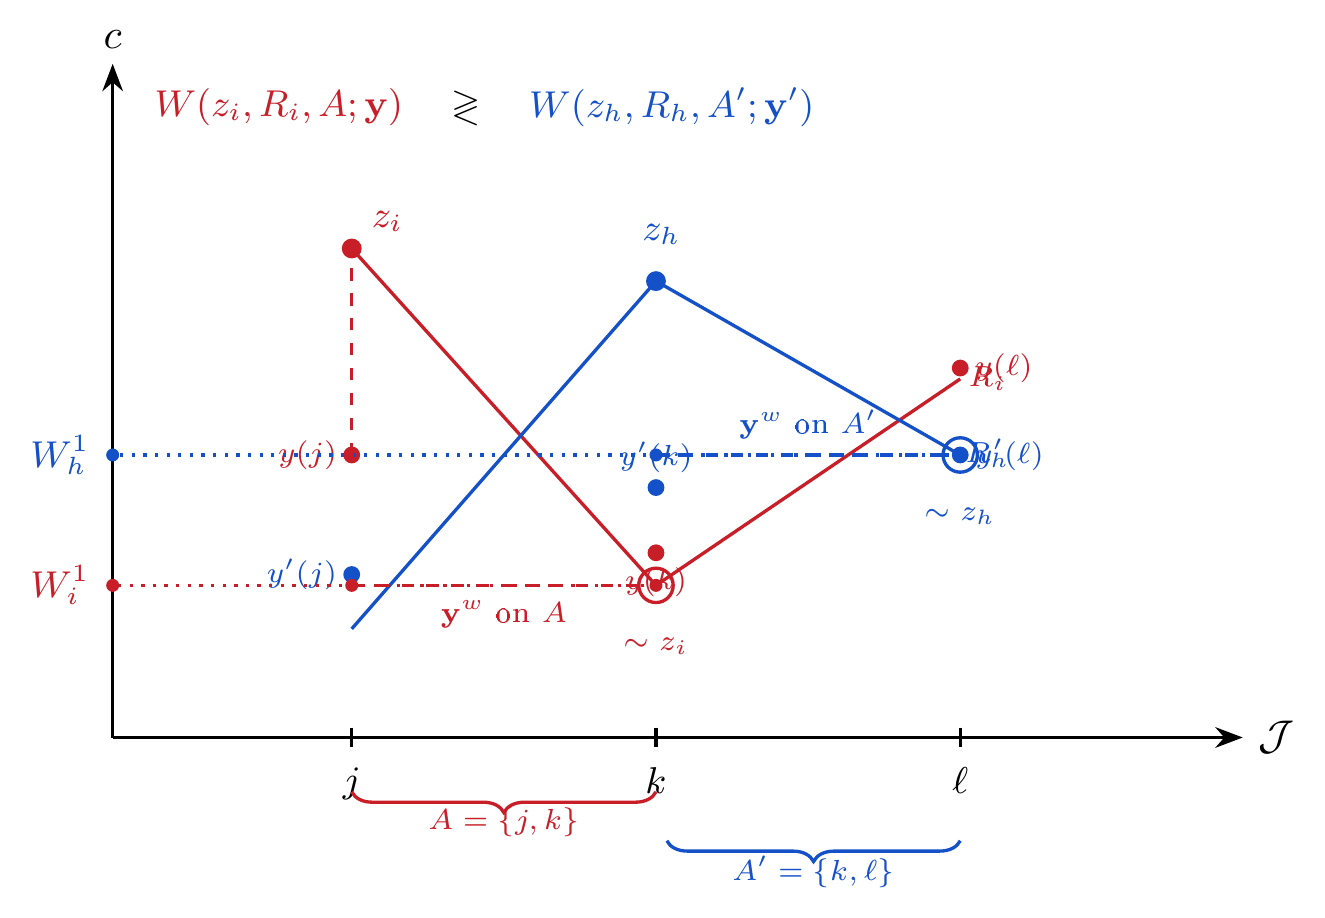
\includegraphics[width=0.95\linewidth,height=\textheight,keepaspectratio,alt={Own-set equal-consumption equivalents. The theoretical W1 construction from the companion theory paper. Individuals with preferences R\_i,R\_h and ability sets A=\textbackslash\{j,k\textbackslash\} and A\^{}\{\textbackslash prime\}=\textbackslash\{k,\textbackslash ell\textbackslash\} attain z\_i and z\_h. For each individual, a common consumption level is assigned to every job in their own set; the level at which the preferred reference job becomes indifferent to the attained bundle is the money metric. Adapted from Haydar and Maniquet (2026), work in progress. This is the deterministic construction; the estimated measure is its ex-ante extension, defined in Section 4.}]{figures/v5/theory_w1.png}
\caption{\textbf{Own-set equal-consumption equivalents.} The theoretical W1 construction from the companion theory paper. Individuals with preferences \(R_i,R_h\) and ability sets \(A=\{j,k\}\) and \(A^{\prime}=\{k,\ell\}\) attain \(z_i\) and \(z_h\). For each individual, a common consumption level is assigned to every job in their own set; the level at which the preferred reference job becomes indifferent to the attained bundle is the money metric. Adapted from Haydar and Maniquet (2026), work in progress. This is the deterministic construction; the estimated measure is its ex-ante extension, defined in Section 4.}
\end{figure}

The first figure depicts the theoretical W1 construction adapted from the companion theory paper by Haydar and Maniquet (2026). It constructs a deterministic own-set equal-consumption equivalent, using each individual's preferred reference job. Section 4 states the empirical implementation on the current estimated model -- a home-reference simplification that holds because staying at home maximises the non-consumption index for every household in both samples -- and derives its closed form; the deterministic figure does not depict an estimated welfare result.

One comparative static is worth stating plainly at the outset, because it is easy to misread. Holding the attained situation fixed, a person with a larger reference menu may need less uniform consumption to reach the same satisfaction. When actual opportunities change, however, both the attainment and the reference menu change. The net effect on equivalent consumption depends on both. Measuring attainment against one's own opportunities is therefore not a claim that larger menus are intrinsically better, and we make no such claim.

\textbf{The empirical approach.} The behavioural half is a random-utility, random-opportunity model of job choice. A job is a package: an employment state, an occupation, a weekly hours arrangement and an hourly wage. Households rank packages by consumption and leisure, and the packages differ in how available they are. Preferences and opportunity components are jointly estimated, with their separation relying on maintained functional-form and exclusion restrictions. Neither is observed as a complete schedule. Every package is priced through the French tax-benefit system, so a change of hours or occupation moves disposable income through the actual schedule of taxes and transfers rather than a linear approximation. We estimate the model separately on 1,540 single-adult and 2,223 couple households drawn from French EU-SILC, with couples choosing jointly under a shared household budget.

A separately defined ex-ante metric is being reconstructed for comparison. Historical ex-ante percentages are not current results and are not shown. The verified attained-bundle measure and its observed-bundle results remain the current welfare evidence; no settled comparison between the two metrics is available.

The computed preliminary restricted-operator decomposition, including all numerical results and their limitations, is reported in Appendix D.

Dispersion in consumption is quantitatively large relative to dispersion in log well-being: \(\operatorname{Var}(\log C)\) is roughly 100--127\% of \(\operatorname{Var}(\log W)\), with the excess offset by a large negative covariance between consumption and the leisure valuation. This bounded decomposition exercise holds household resources, needs and composition fixed, leaving important sources of dispersion outside the P/A/B allocation.

\textbf{Relation to existing work.} Every ingredient here has antecedents, and the contribution is the combination and the empirical answer, not any one step.

Modelling labour supply as choice among latent jobs, with preferences and opportunity components jointly estimated under maintained functional-form and exclusion restrictions, is due to \citet{aaberge1995} and \citet{aaberge1999}, developed by \citet{dagsvikstrom2006} and \citet{dagsvikjia2016}, surveyed by \citet{aaberge2018}, and set out for applied work by \citet{capeau2016}. We inherit that framework, including its distinction between the intensity of an offer and the probability of a choice, and its reliance on excluded opportunity shifters to separate components that choices alone do not separate. \citet{capeau2016} also supply two of the identifying restrictions we maintain: the wage-offer distribution is independent of offered hours, and a local unemployment measure shifts availability while being excluded from preferences. Their Belgian application already covers single women, single men and couples, so covering both household types is not itself a contribution.

Combining such a model with a monetary welfare evaluation is also established. \citet{aaberge1995} translate attained utility into an equivalent income against a stated reference household, choice set and tax system, and \citet{aaberge2004} evaluate reforms with joint household choice and restricted hours. \citet{jiathoresen2021} make the case for the job-choice model in exactly this role and report a distribution of compensating variation for a Norwegian reform, and \citet{jacquet2026} compare a standard compensating variation with one computed after replacing preference characteristics by reference values. All four evaluate a \emph{change} between policy regimes. Our object is a cross-sectional distribution of levels under one policy system, and its attribution. A reform gain and a level have different origins and different denominators; a small preference-related reform difference would not imply a small preference share in our decomposition, and our shares do not estimate their reform gains.

The normative half draws on the literature that refuses to resolve interpersonal comparison by assuming common preferences. \citet{fleurbaeymaniquet2006}, \citet{fleurbaeymaniquet2017} and \citet{fleurbaeymaniquet2018} set out how a reference bundle encodes a position on compensation and responsibility; \citet{decosterhaan2015} and \citet{bargain2013} show empirically how much a welfare ordering moves with that choice. Their references fix a wage or an unearned-income intercept and maximize over a deterministic budget set. Ours fixes consumption across the alternatives of an estimated opportunity distribution and integrates. That is a different reference and, as Section 6 records, the ordering is sensitive to it.

The closest decomposition precedents are two. \citet{muehlhan2023} combines a structural labour-supply model with involuntary-unemployment restrictions and a Shapley attribution, decomposing the change in German household \emph{income} inequality into temporal factors and binary restrictions. \citet{creedyherault2011}, in the section that constructs money-metric distributions under alternative policy and population states, decompose a change in inequality and social welfare by averaging over the two orders in which policy and population can be changed; theirs is the closest money-metric welfare-inequality decomposition we know. Both are decompositions of a \emph{change} between two situations, with policy, population or temporal factors as the factors. Ours is a decomposition of a cross-sectional \emph{level} of well-being inequality, with the factors defined as structural operators inside an estimated job-choice model: what a household prefers, which jobs it can reach, what those jobs pay, and what its budget and needs are. The wider behavioural-simulation decomposition tradition, \citet{bargain2012} and \citet{jessen2019}, decomposes income changes in the same spirit.

The allocation rule is inherited outright. \citet{shorrocks1982} states the accounting requirements a decomposition should satisfy; \citet{shorrocks2013} places the Shapley value at the centre of distributional decomposition; \citet{sastretrannoy2002} documents how much the answer can depend on how the exercise is set up. The preliminary three-operator exercise in Appendix D needs no grouping and uses the plain Shapley value on a three-player game. We claim no new allocation principle. Complete recomputation of every coalition, rather than a linear approximation, likewise has precedents and is better described as methodological discipline than as a contribution.

What is new, to our knowledge, is the conjunction: a random-utility random-opportunity model of job choice, an opportunity-sensitive money-metric welfare level built on the own-set equal-consumption principle, and a bounded, preliminary structural game over systematic utility heterogeneity, coarse geographic/temporal access heterogeneity and earning opportunities, with complete recomputation of welfare and inequality under every coalition. The application-specific methodological contribution is the game and its counterfactual operators, reported as preliminary and work in progress pending the counterfactual-attainment estimand of Section 4. The cooperative-game allocation rule is inherited.

\textbf{Roadmap.} Section 2 describes the data and the household budget construction. Section 3 presents the latent-jobs model, its identifying restrictions and its estimation. Section 4 defines the money-metric welfare measure and the structural decomposition. Section 5 reports the behavioural and welfare results for both household types. Section 6 examines sensitivity and states the limitations. Section 7 concludes.

\section{Data}\label{data}

The data are French EU-SILC, collection year 2016, with income reference year 2015. Taxes, benefits and disposable income are computed by EUROMOD \citep{sutherlandfigari2013} under the French 2015 policy system, which is the system in force over the income reference period. We use the same three dates consistently: the survey is collected in 2016, incomes refer to 2015, and the simulated policy system is 2015.

\subsection{The estimation samples}\label{the-estimation-samples}

\Needspace*{12\baselineskip}\small\setlength{\tabcolsep}{3pt}\begin{longtable}[]{@{}
  >{\raggedright\arraybackslash}p{(\linewidth - 4\tabcolsep) * \real{0.3333}}
  >{\raggedright\arraybackslash}p{(\linewidth - 4\tabcolsep) * \real{0.3333}}
  >{\raggedright\arraybackslash}p{(\linewidth - 4\tabcolsep) * \real{0.3333}}@{}}
\caption{Sample construction. Unweighted households remaining after each screen, from the France 2016 EUROMOD input file to the two estimation samples. Rows are sequential; the counts are read from the frame records and are not reconstructed by subtraction.}\tabularnewline
\toprule\noalign{}
\begin{minipage}[b]{\linewidth}\raggedright
Screen
\end{minipage} & \begin{minipage}[b]{\linewidth}\raggedright
Single-adult
\end{minipage} & \begin{minipage}[b]{\linewidth}\raggedright
Couple
\end{minipage} \\
\midrule\noalign{}
\endfirsthead
\toprule\noalign{}
\begin{minipage}[b]{\linewidth}\raggedright
Screen
\end{minipage} & \begin{minipage}[b]{\linewidth}\raggedright
Single-adult
\end{minipage} & \begin{minipage}[b]{\linewidth}\raggedright
Couple
\end{minipage} \\
\midrule\noalign{}
\endhead
\bottomrule\noalign{}
\endlastfoot
the raw France 2016 input file & 4,038 & 5,965 \\
one- or two-adult households (composition screen) & 4,038 & 5,965 \\
every adult aged 20 to 60 & 2,131 & 3,662 \\
no adult still in education & 2,036 & 3,521 \\
no old-age, disability or survivor pension receipt & 1,755 & 3,218 \\
labour status in scope & 1,598 & 2,412 \\
no other employable or earning member & 1,564 & 2,323 \\
observed hours and wage inside the calibrated support & 1,555 & 2,275 \\
hours outside {[}5,70{]} or unsupported military occupation (ISCO 0) on an employed decider & 1,543 & 2,223 \\
observed chosen alternative priced at non-positive disposable consumption & 1,540 & 2,223 \\
\textbf{Estimation sample} & \textbf{1,540} & \textbf{2,223} \\
\end{longtable}

The screens are of three kinds and it is worth separating them. The first two define the decision unit: the household must contain either one unpartnered adult or two mutually linked adults of opposite sex, and every decider must be between twenty and sixty. This is the largest exclusion and it is structural. Multi-generational households, flat-shares, adult children living with parents and same-sex couples are outside the estimated population, and no result extends to them. Because the age screen binds on both spouses, it removes proportionally more couples than singles.

The second kind removes households for whom the model does not define an offer set: adults in full-time education, households receiving an old-age, disability or survivor pension, and deciders whose labour-market status lies outside employment, unemployment and inactivity. Together with the pension screen this is why the surviving employment rate is high. The employment share below should be read as a share among people for whom working is a live option, not as a French employment rate.

The third kind is support. An employed decider's observed hours must lie in the closed interval \([5, 70]\) hours per week and the delivered hourly wage in \([2, 590]\) euros per hour, because those are the boundaries of the supports the opportunity densities are defined on. An observed occupation must map into the four modelled groups; ISCO 0, the armed forces, does not, and the resulting exclusion is \emph{unsupported} occupation, not missing occupation. Three single-adult households whose own observed job prices to non-positive disposable consumption are removed, because the log-consumption term is undefined at their observed choice; non-positive \emph{simulated} alternatives receive a one-euro consumption floor before utility is evaluated. Those are sampled alternatives entering the estimated choice likelihood. They do not enter the welfare measure of Section 4, which evaluates only each household's own observed job and its home state, both already screened to strictly positive consumption.

\Needspace*{12\baselineskip}\small\setlength{\tabcolsep}{3pt}\begin{longtable}[]{@{}
  >{\raggedright\arraybackslash}p{(\linewidth - 4\tabcolsep) * \real{0.3333}}
  >{\raggedright\arraybackslash}p{(\linewidth - 4\tabcolsep) * \real{0.3333}}
  >{\raggedright\arraybackslash}p{(\linewidth - 4\tabcolsep) * \real{0.3333}}@{}}
\caption{The four occupation groups. ISCO-08 major groups are aggregated into four modelled groups; group 1 is the omitted reference in the estimated occupation block. This is a research aggregation adopted for this paper, not an ILO classification. ISCO 0, the armed forces, has no modelled alternative and is a sample screen; that is unsupported occupation, not missing occupation.}\tabularnewline
\toprule\noalign{}
\begin{minipage}[b]{\linewidth}\raggedright
Model group
\end{minipage} & \begin{minipage}[b]{\linewidth}\raggedright
ISCO-08 major groups
\end{minipage} & \begin{minipage}[b]{\linewidth}\raggedright
Description
\end{minipage} \\
\midrule\noalign{}
\endfirsthead
\toprule\noalign{}
\begin{minipage}[b]{\linewidth}\raggedright
Model group
\end{minipage} & \begin{minipage}[b]{\linewidth}\raggedright
ISCO-08 major groups
\end{minipage} & \begin{minipage}[b]{\linewidth}\raggedright
Description
\end{minipage} \\
\midrule\noalign{}
\endhead
\bottomrule\noalign{}
\endlastfoot
1 (reference) & 6--9 & Skilled agricultural, craft, plant and machine operators, and elementary occupations \\
2 & 5 & Service and sales workers \\
3 & 4 & Clerical support workers \\
4 & 1--3 & Managers, professionals, technicians and associate professionals \\
\end{longtable}

\subsection{What the households look like}\label{what-the-households-look-like}

\Needspace*{12\baselineskip}\small\setlength{\tabcolsep}{3pt}\begin{longtable}[]{@{}>{\RaggedRight\arraybackslash}p{0.2500\linewidth}>{\RaggedRight\arraybackslash}p{0.2247\linewidth}>{\RaggedRight\arraybackslash}p{0.2247\linewidth}>{\RaggedRight\arraybackslash}p{0.2247\linewidth}@{}}
\caption{Descriptive means on the estimation samples. Weighted by the household cross-sectional weight; one row per household, with spouse-specific variables carried on the household row. Hours and wages are conditional on employment. These are observed inputs, not model predictions.}\tabularnewline
\toprule\noalign{}
Measure & Single-adult decider & Couple man & Couple woman \\
\midrule\noalign{}
\endfirsthead
\toprule\noalign{}
Measure & Single-adult decider & Couple man & Couple woman \\
\midrule\noalign{}
\endhead
\bottomrule\noalign{}
\endlastfoot
Age (years) & 41.1 & 39.8 & 37.8 \\
Children under 20 & -- & -- & -- \\
Usual weekly hours, employed & 37.6 & 41.1 & 35.8 \\
Delivered hourly wage, employed (EUR/hour) & -- & -- & -- \\
Households (unweighted) & 1,540 & 2,223 & \\
\end{longtable}

\begin{figure}[H]
\centering
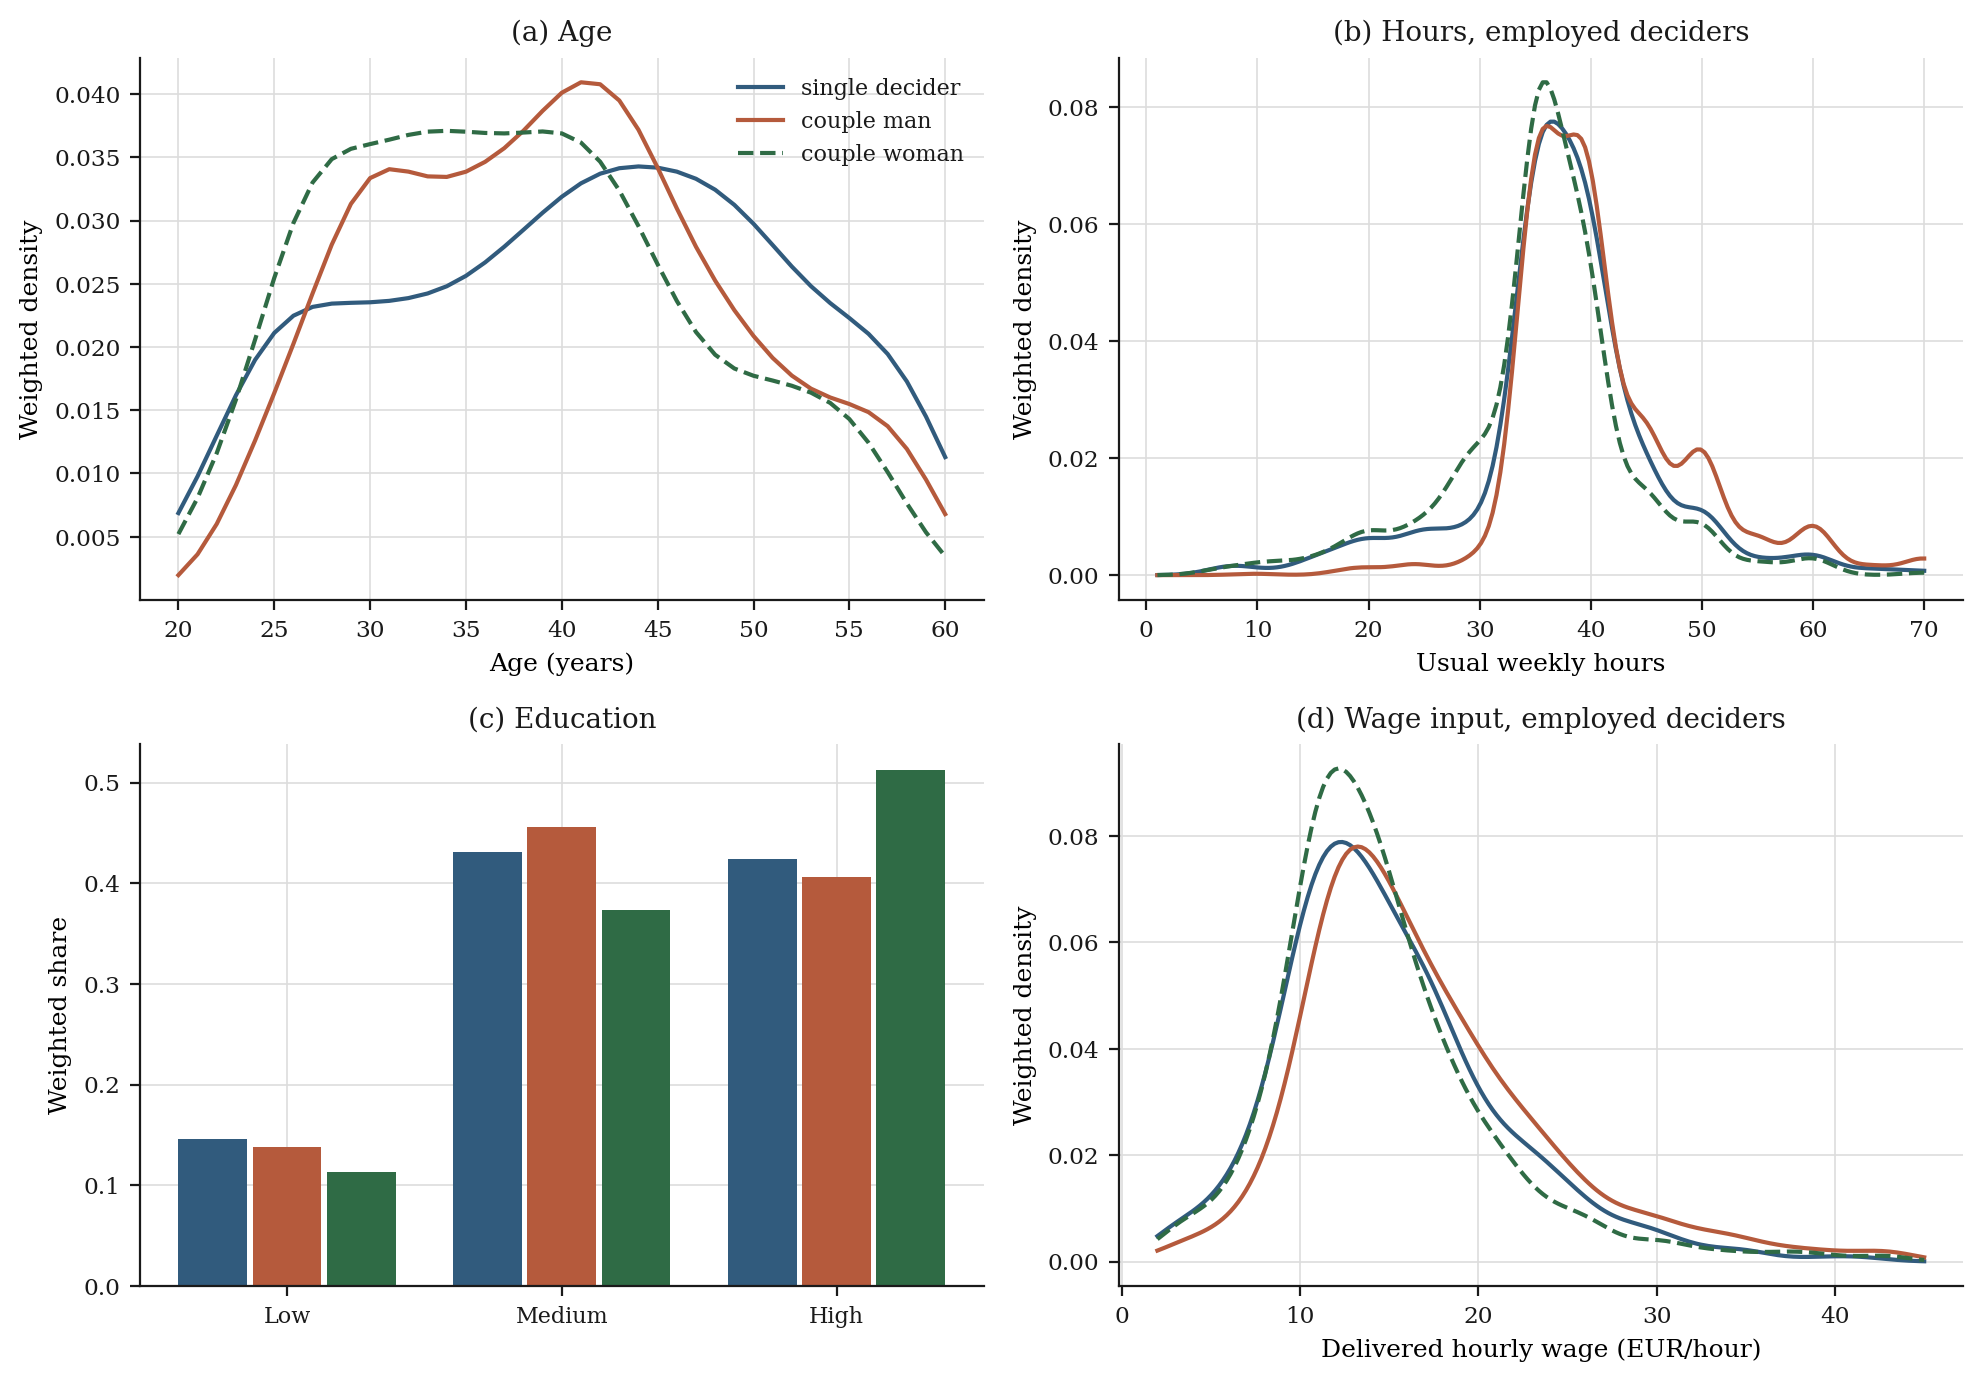
\includegraphics[width=0.95\linewidth,height=\textheight,keepaspectratio,alt={Weighted distributions on the estimation samples: age, usual weekly hours among employed deciders, education, and the delivered hourly wage input. Observed inputs, not model predictions.}]{figures/v5/figV08_data_panel.png}
\caption{Weighted distributions on the estimation samples: age, usual weekly hours among employed deciders, education, and the delivered hourly wage input. Observed inputs, not model predictions.}
\end{figure}

Education is the three-level ISCED grouping, with the medium level as the omitted reference in the wage equation. Potential experience is years since leaving education, entering the wage equation in units of 20 years, with the square recomputed after scaling rather than carried forward. A child is any resident household member under 20, counted without a parent link. Age enters preferences centred on the sample mean decider age and divided by 10 years.

\Needspace*{12\baselineskip}\small\setlength{\tabcolsep}{3pt}\begin{longtable}[]{@{}>{\RaggedRight\arraybackslash}p{0.2500\linewidth}>{\RaggedRight\arraybackslash}p{0.1650\linewidth}>{\RaggedRight\arraybackslash}p{0.1650\linewidth}>{\RaggedRight\arraybackslash}p{0.1650\linewidth}>{\RaggedRight\arraybackslash}p{0.1650\linewidth}@{}}
\caption{Observed joint participation regimes among the 2,223 estimated couple households. These are joint regimes, not two spouse marginals.}\tabularnewline
\toprule\noalign{}
Regime & Meaning & Weighted share & Mean hours, man & Mean hours, woman \\
\midrule\noalign{}
\endfirsthead
\toprule\noalign{}
Regime & Meaning & Weighted share & Mean hours, man & Mean hours, woman \\
\midrule\noalign{}
\endhead
\bottomrule\noalign{}
\endlastfoot
BB & both spouses employed & 0.8435 & 41.0 & 35.9 \\
MO & man employed, woman not employed & 0.0796 & 41.5 & 0.0 \\
WO & woman employed, man not employed & 0.0547 & 0.0 & 35.0 \\
NN & neither spouse employed & 0.0222 & 0.0 & 0.0 \\
\end{longtable}

\subsection{The household budget}\label{the-household-budget}

For a given work arrangement the tax-benefit model is given the implied gross labour inputs, weekly hours, hourly wage, and earnings split at the thirty-five hour threshold, together with the household's non-labour inputs and roster, and returns disposable income. Only deciders receive counterfactual overrides; other members keep their baseline values. The accounting identity linking original income, benefits, taxes and social contributions to disposable income holds to machine precision at both the person and the household-alternative level, before and after the benefit take-up adjustment. Disposable income is summed over all resident members of the household.

\begin{figure}[H]
\centering
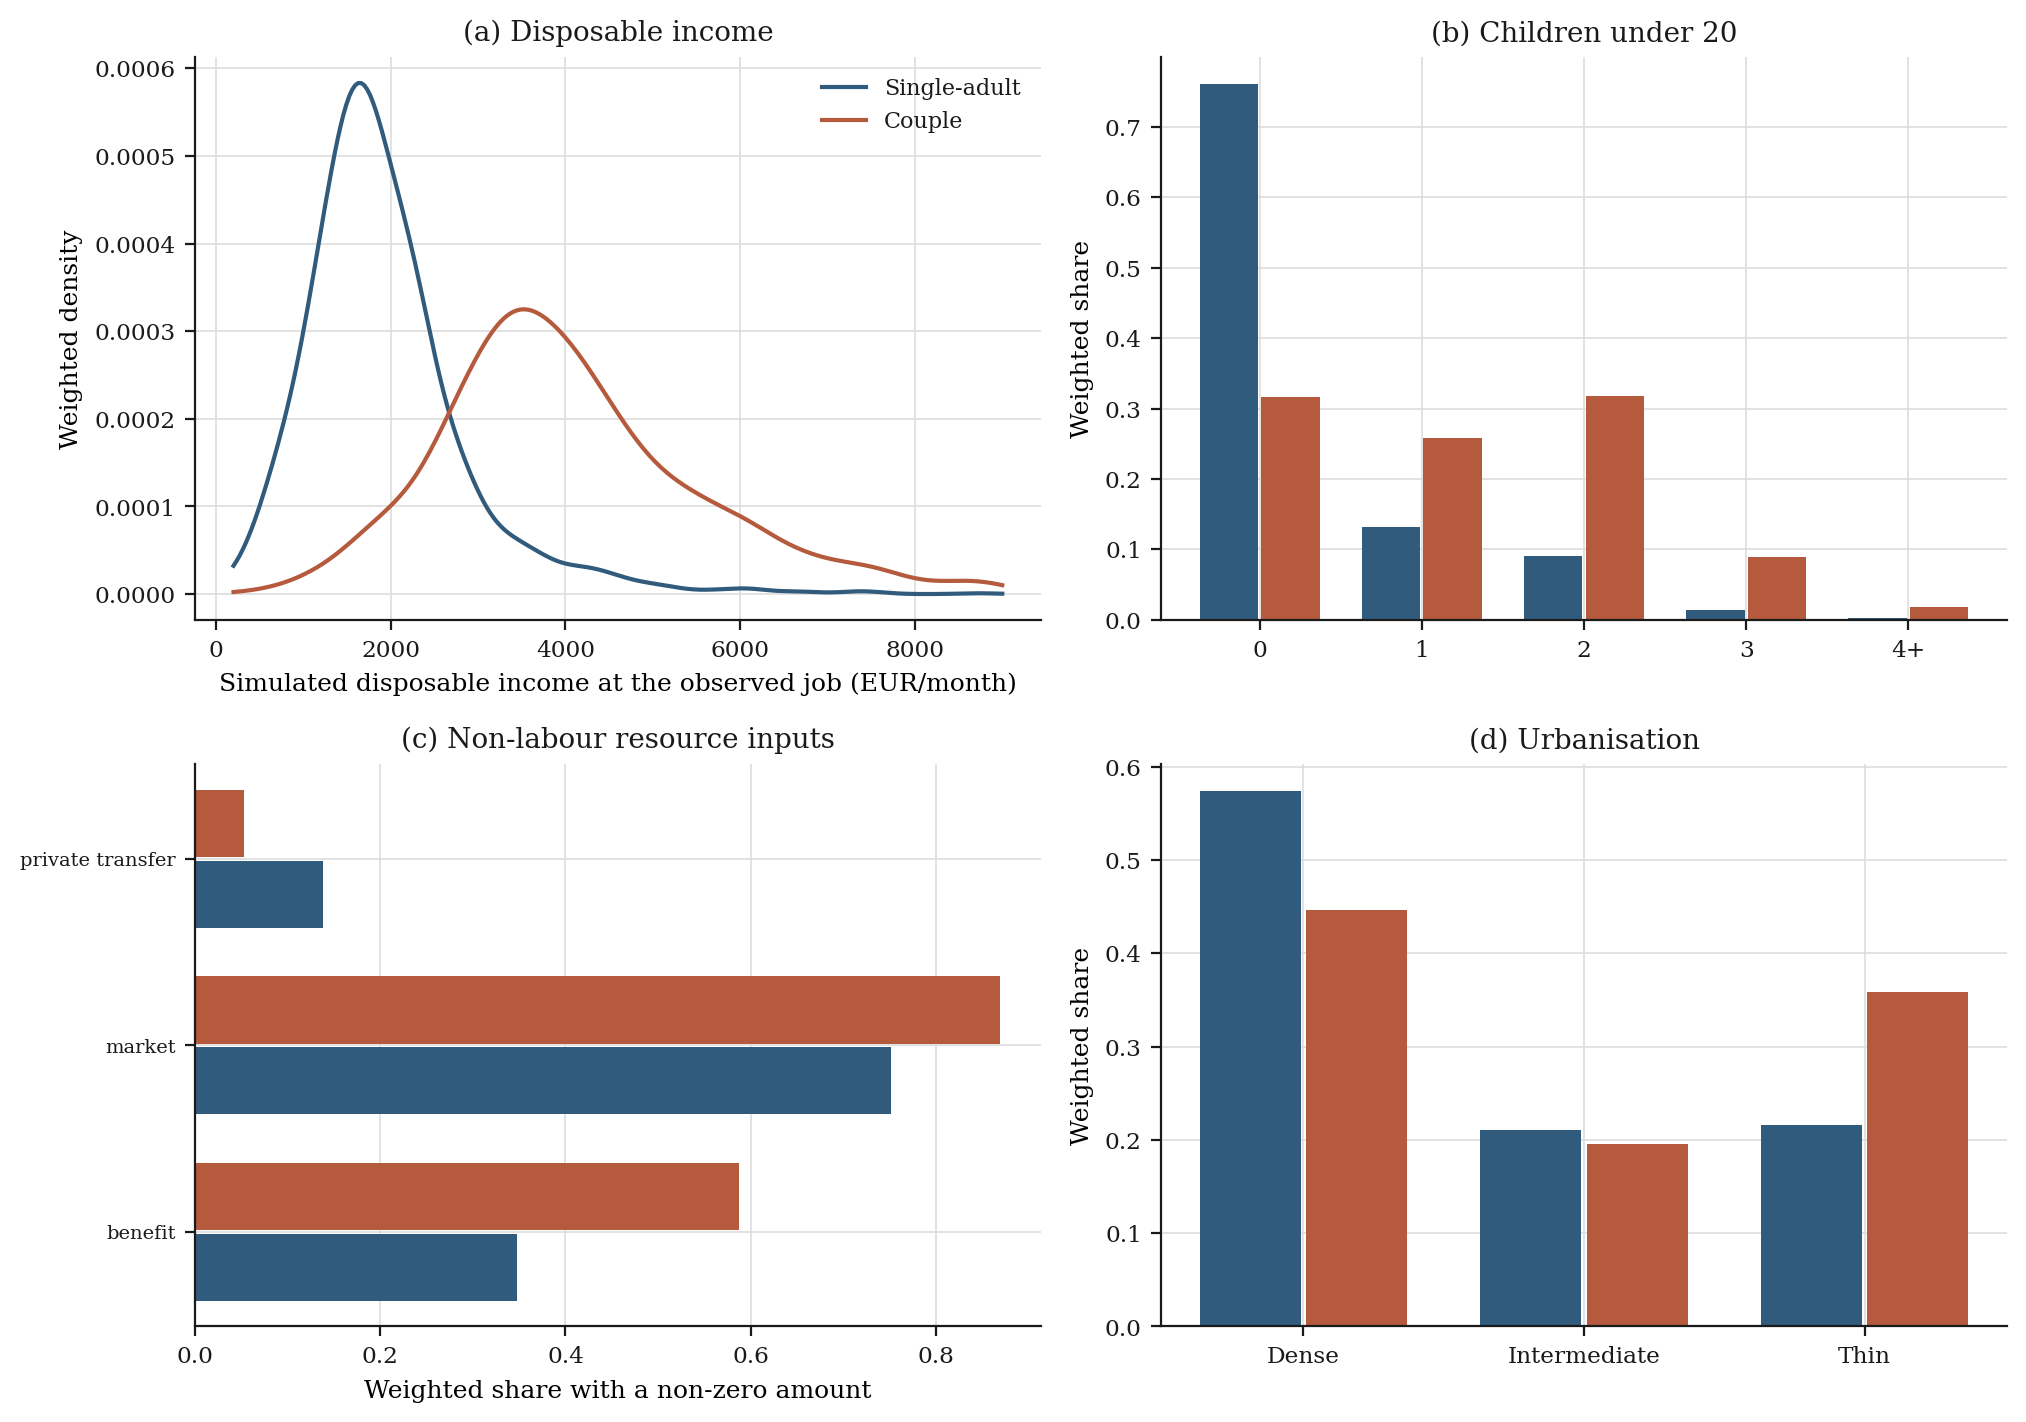
\includegraphics[width=0.95\linewidth,height=\textheight,keepaspectratio,alt={Weighted distributions on the estimation samples: simulated disposable income at the observed job, children under twenty, the incidence of non-labour budget inputs by family, and urbanisation. Panel (a) is a tax-benefit output evaluated at the observed choice; panel (c) reports inputs to that calculation. The two are never added, and stocks are never summed with monthly flows.}]{figures/v5/figV09_resources_panel.png}
\caption{Weighted distributions on the estimation samples: simulated disposable income at the observed job, children under twenty, the incidence of non-labour budget inputs by family, and urbanisation. Panel (a) is a tax-benefit output evaluated at the observed choice; panel (c) reports inputs to that calculation. The two are never added, and stocks are never summed with monthly flows.}
\end{figure}

Panel (c) of the figure reports the \emph{incidence} of non-labour budget inputs by family, not a cash total. Some of these are stocks, some are annual flows and some are monthly; they are inputs to the tax-benefit calculation and are not added together into one income concept. The pension family is empty by construction, because pension receipt is a sample screen. Panel (a) reports the tax-benefit \emph{output} at the observed job, which is an object of a different kind and is never added to panel (c).

Local labour-market conditions enter through a group unemployment measure, a population-weighted exposure index for the decider's region and age-education cell, stored as a fraction and entering the employment index multiplied by 10. Regional and urbanisation variation supports the access specification conditional on the exclusion restriction and the functional form; it does not by itself identify access, and no causal effect of geography is claimed anywhere in this paper.

\section{A latent-jobs model of household labour supply}\label{a-latent-jobs-model-of-household-labour-supply}

A job is a package \(j\): an employment state \(e\in\{0,1\}\) and, when employed, an occupation \(k\in\{1,\dots,4\}\), weekly hours \(h\in[5,70]\) and an hourly wage \(w\in[2,590]\). The base measure \(\nu\) places counting mass on the single non-employment point and, on the employed part, counting measure over occupations with Lebesgue measure over hours and wages. A household chooses one package; a couple chooses one pair of packages under a shared budget.

\subsection{Preferences}\label{preferences}

Let \(C_i(j)\) be priced monthly disposable consumption at \(j\) and \(\ell_i(j)\) normalized leisure, \((80-h)/10\) hours per week, floored at one hour. For a single adult of sex group \(g\), deterministic utility is

\[
u_{ij}=\underbrace{\beta_{\ell}^{g}(\mathbf x_i)\;
\mathcal B\!\left(\tilde\ell_{ij};\theta_{\ell}^{g}\right)}_{L_{ij}}
\;+\;\beta_c\log\tilde c_{ij},
\qquad
\beta_{\ell}^{g}(\mathbf x_i)=\beta_{\ell 0}^{g}+\beta_{\ell a}^{g}a_i
+\beta_{\ell a^{2}}^{g}a_i^{2}
+\mathbb 1\{g=\text{women}\}\,\beta_{\ell k}^{g}k_i,
\]

where \(\mathcal B(z;\theta)=(z^{\theta}-1)/\theta\) with \(\mathcal B(z;0)=\log z\), \(\tilde\ell_{ij}\) is normalized leisure, \(\tilde c_{ij}=C_{ij}/\lambda_c\), \(a_i\) is centred age in decades and \(k_i\) is the child count. For a couple the index is additive across spouses with no direct cross-leisure term,

\[
u_{ij}=\beta_{\ell}^{m}(\mathbf x_i)\,\mathcal B(\tilde\ell^{m}_{ij};\theta_{\ell}^{m})
      +\beta_{\ell}^{f}(\mathbf x_i)\,\mathcal B(\tilde\ell^{f}_{ij};\theta_{\ell}^{f})
      +\beta_c\log\tilde c_{ij},
\]

with consumption the tax-unit sum over all members. We write \(L_i(j)\) throughout for the complete non-consumption part of the index, which for a couple contains both leisure terms.

The systematic leisure specification is not age alone: it carries an intercept, age, age squared and group-specific leisure curvature for each of the four adult groups, plus a number-of-children shifter for women; sex and household type are carried by separate parameter blocks. ``The baseline deliberately keeps systematic preference heterogeneity parsimonious: age profiles for all four adult groups and a child-related shifter for women. The child term is interpreted as a reduced-form behavioural/time-constraint shifter, not as pure taste.''

Three features of this specification are decisions and are worth naming. The consumption curvature is exactly zero, so the consumption term is \(\beta_c\log(C/\lambda_c)\) and the marginal utility of consumption is \(\beta_c/C\), independent of the normalizer. The consumption weight \(\beta_c\) is \textbf{estimated}, not fixed at one. And the random-utility shock is i.i.d. type-I extreme value with scale one, so utility is measured in the natural unit of that scale. Fixing the shock scale is a normalization; additionally fixing \(\beta_c\) would be a substantive restriction relative to that normalization, and estimating \(\beta_c\) removes it. Neither step identifies an absolute cardinal utility scale, and fixing the consumption functional form is not by itself what identifies the shock scale.

The normalizer \(\lambda_c\) is a units convention. Under exact log consumption it enters the index as the alternative-invariant constant \(-\beta_c\log\lambda_c\), so it cancels from every choice probability; it does not appear in the welfare measure of Section 4 at all.

\subsection{Opportunities}\label{opportunities}

The opportunity density gives the relative intensity with which packages are available to household \(i\), before any choice is made. It is a product of \textbf{four} factors, switched off on non-employment by the employment indicator \(E_{ij}=\mathbb 1\{h_{ij}>0\}\):

\[
g_{ij}=g^{E}_{ij}\cdot\left(g^{H}_{ij}\cdot g^{\mathrm{Occ}}_{ij}\cdot g^{W}_{ij}\right)^{E_{ij}} .
\]

\textbf{Access}, \(g^{E}_{ij}=\exp\{\beta_E+\beta_s s_i+\sum_{r=2}^{8}\beta_r\,\mathrm{reg}_{ir}+\beta_u u_i+\beta_m m_i\}\), carries the local group unemployment measure \(s_i\), the region indicators and urbanisation, and is the factor inside which local-market access lives. \textbf{Hours}, \(g^{H}_{ij}=\exp\{\sum_b \beta_b\mathbb 1\{h_{ij}\in b\}\}\), elevates five bands over a residual reference set of total width 26.5 hours per week, so every band coefficient is read against that residual and none of the five is normalized to zero; the narrow full-time band \([33.5,36.5)\) is a density elevation over an interval, not an atom at thirty-five hours. \textbf{Occupation}, \(g^{\mathrm{Occ}}_{ij}=\exp\{\beta^{\mathrm{occ}}_{k,g}\}\) with \(\beta^{\mathrm{occ}}_{1,g}\equiv 0\). \textbf{Wage offer}, \(g^{W}_{ij}\), is log-normal with location \(\mu_i=\beta_{w0}+\beta_{wL}L_i+\beta_{wH}H_i+\beta_{wx}x_i+\beta_{wx^{2}}x_i^{2}+\delta_{\mathrm{occ}}\) and dispersion \(\sigma\), truncated to \([2,590]\) euros per hour and renormalized on that support.

Two properties of the normalization matter later, for estimation and for the identification argument below. Write \(\widehat g_{ij}=g_{ij}/Z_i\) for the density normalized to unit mass on the whole package space. The wage factor integrates to one \emph{conditional on employment and occupation}, because the truncated density is renormalized on its own support; and the non-consumption index \(L_{ij}\) has no wage argument. The pay-neutrality property of the welfare reference established in Section 4 rests on a simpler fact than either of these: the reference job itself, staying at home, carries no opportunity-density argument at all, so none of \(g\), the proposal, the shock or an intensity parameter enters the reference.

The full opportunity model contains employment access, hours, occupation and wage-offer blocks. This bounded decomposition exercise does not equalise all of them: its \(A\) channel is limited to local geographic/temporal access shifters (region, urban/rural, year), while personal occupation access, hours-band access and other alternative characteristics remain fixed; \(B\) carries earning opportunities.

\subsection{Identification, in words}\label{identification-in-words}

Choices alone do not separate a taste for leisure from a scarcity of jobs at that number of hours. Three kinds of restriction do the work. Preferences are smooth in hours through the leisure index, while the opportunity density is a step function over bands, so a spike in observed hours at a band is read as availability rather than as a kink in tastes. Excluded shifters enter availability and not preferences: the local group unemployment measure and the regional and urbanisation indicators shift the employment index and appear nowhere in utility. And the wage-offer distribution is specified as independent of offered hours conditional on occupation, which separates the wage location from the hours density. These are the restrictions of \citet{capeau2016} and \citet{dagsvikjia2016}, maintained here rather than tested. The regional variation supports the access block conditional on those restrictions; it does not establish separate identification on its own, and it is not a causal design.

Preferences and opportunity components are jointly estimated, with their separation relying on maintained functional-form and exclusion restrictions. No causal interpretation is attached to that separation.

\subsection{Estimation}\label{estimation}

The choice set is a continuum, so the likelihood is evaluated over sampled alternatives. For each household we draw \(R=100\) alternatives from a proposal density \(q_{ij}\) and place the observed package in the set as well, giving a set \(\mathcal C_i\) with \(|\mathcal C_i|=101\) rows. Write the sampled-set index

\[
V_{ij}=u_{ij}+\log g_{ij}-\log q_{ij},
\qquad
q_{ij}=q^{E}_{ij}\left(q^{H}_{ij}q^{W}_{ij}q^{\mathrm{Occ}}_{ij}\right)^{E_{ij}} .
\]

The contribution of household \(i\) is then the conditional probability of its observed package \(y\) within that set,

\[
\Pr\!\left(y\mid\mathcal C_i\right)=
\frac{n_{y}\exp V_{iy}}{\sum_{s\in\mathcal C_i}\exp V_{is}} .
\]

The denominator runs over slots rather than distinct packages, and a package drawn more than once keeps its multiplicity, \(n_y\); the observed package carries the same proposal correction as any other row. The proposal density is a computational device and never an economic object: it is not an offer, an availability or an opportunity. The proposal is fitted out of fold, so a household's own outcome never enters the proposal used to score it. For couples the proposal draws the joint participation regime first and then the two spouse packages conditional on it.

Standard errors are cluster-robust on the household. Optimization uses five starts under two polishing contracts, ten terminal paths in all; we report the spread of the criterion across those paths and the eigenvalues of the exact Hessian at the selected optimum. Those diagnostics support a stable local solution found from the starts tested. They are not a proof of global uniqueness, and we do not claim one.

Two features of the observation rule remain genuinely open and are stated here rather than in a footnote. The sample screens on the observed hours and wage of employed deciders, so the estimation sample is selected on an outcome of the process being modelled. The conditional likelihood above is the correct object for a sampled choice set; it is not automatically the correct object for an outcome-selected sample, and we have not established which correction, if any, the screen requires. Separately, the derivation of the sampled-set probability conditions on a labelled collection of slots; small observed cross-coordinate correlations and a binomial-looking multiplicity distribution are consistent with independent draws but do not by themselves establish the sampling law. Both are recorded as unresolved in Section 6.

\section{Money-metric well-being and structural inequality decomposition}\label{money-metric-well-being-and-structural-inequality-decomposition}

\subsection{\texorpdfstring{The verified own-set equal-consumption \(W^1_F\) construction}{The verified own-set equal-consumption W\^{}1\_F construction}}\label{the-verified-own-set-equal-consumption-w1_f-construction}

The welfare measure is the amount of consumption that, paid at the fixed non-employment reference \(o\), leaves the household exactly as well off as at its attained situation:

\[
W^1_{i,F}=m_i(o;z_i), \qquad u_i\big(m_i(o),o\big)=u_i(z_i).
\]

This is the theoretical own-set equal-consumption criterion above, \(u_i(z_i)=\max_{j\in A_i}u_i(W_i,j)\), specialised to the reference job \(o\) that the maximisation over the household's own reachable set actually selects. On the current empirical domain the selected reference job is always staying at home: for every household in both samples, non-employment maximises the non-consumption index, so the maximisation collapses to a single evaluation at the household's own observed job against its own home state, \(o\). Under the log-consumption specification of Section 3 this gives the closed form

\[
\boxed{\;W^1_{i,F}=C_i^{\mathrm{obs}}\exp\!\left[\frac{L_i(j_i^{\mathrm{obs}})-L_i(o)}{\beta_c}\right],\;}
\]

where \(C_i^{\mathrm{obs}}\) is the household's own priced disposable consumption at its observed job, \(L_i(j_i^{\mathrm{obs}})\) and \(L_i(o)\) are the non-consumption index at the observed job and at the home state, and \(\beta_c\) is the estimated consumption weight. Four objects do not enter this construction at all: the opportunity density \(\widehat g\), the numerical proposal \(q\), the behavioural shock, and any latent-set intensity parameter -- opportunities act on this measure only through the attained bundle \(j_i^{\mathrm{obs}}\), never through an average or an integral over jobs the household did not take. That home always maximises the non-consumption index, so that \(W^1\) coincides here with the staying-home equivalent, is an empirical-domain property of this specification and this estimated model, verified directly rather than assumed; it is not a theorem of the Haydar-Maniquet framework, which defines the reference job \(o\) as whichever job the maximisation selects and does not guarantee it is staying at home.

The construction is independently verified. A reconstruction that does not import the production code reproduces every pre-registered check -- non-workers equal their own observed consumption exactly, workers strictly below it, no route by which \(\widehat g\), \(q\), the shock, or an intensity parameter can enter -- and reproduces the sample aggregates for both populations to machine precision, confirmed by an independent reimplementation.

\subsection{What the reference does and does not do to pay}\label{what-the-reference-does-and-does-not-do-to-pay}

The money metric is derived from the own-set equal-consumption principle. Under the current empirical specification its direct reference collapses to the universally available non-employment state; opportunity heterogeneity therefore affects the current welfare measure through attained bundles.

The reference does not depend directly on pay. The construction's home reference is a fixed singleton state whose systematic utility carries no opportunity-density, proposal, behavioural-shock or intensity argument, so none of those four objects enters it at all.

Changes in earning opportunities nevertheless change the measure, because they change what the household attains, not the reference it is compared against. The correct statement is therefore narrow and we make only it: \emph{the reference is directly pay-neutral, and earning opportunities reach the measure through the attained evaluation.} We do not report a magnitude for that attained-side channel here: quantifying it under a counterfactual equalization of earning opportunities is a decomposition question, and Appendix D reports only the bounded, preliminary exercise available for that. A qualitative channel existing does not establish that the deterministic independence-of-pay axiom fails for this stochastic functional. That would require fixing the primitives the axiom holds fixed and proving the property, which we have not done and do not claim.

\subsubsection{A worked illustration, in the current construction}\label{a-worked-illustration-in-the-current-construction}

Not a description of any real household. For a one-nat shortfall, \(L_i(j_i^{\mathrm{obs}})-L_i(o)=-1\), the closed form gives \(W^1_{i,F}=C_i^{\mathrm{obs}}\exp(-1/\beta_c)<C_i^{\mathrm{obs}}\). Current nonworkers: \(W=C\). Current workers: \(W<C\) under the maintained empirical domain. This is a mechanical illustration of the closed form, not an empirical claim about any particular household.

\subsection{Interpersonal comparison and the unit}\label{interpersonal-comparison-and-the-unit}

The measure is defined at the household. Comparing households of different size requires an equivalence scale, which is a normative choice and not an estimate. We report every result on two bases: a raw household basis, and an equivalized basis using the modified OECD scale. We never pool the two household types into one distribution, because the two applications carry different reference constructions and the levels are not comparable; every share below is a share of the baseline inequality of its own population.

The restricted counterfactual operators and allocation rule are set out in Appendix D.

\section{Empirical results}\label{empirical-results}

\subsection{Behavioural estimates}\label{behavioural-estimates}

The estimated model has 41 free coordinates for single adults, of which 40 are interior, and 47 for couples, all interior. The criterion is 6253.463 and 10283.034 respectively. Across ten terminal paths from five starts under two polishing contracts, the criterion varies by 1.1e-10 for single adults and 1.3e-09 for couples, and the smallest eigenvalue of the exact Hessian on the interior block is 0.1669 and 0.0771. One single-adult coordinate, the female age-square term in the leisure weight, sits at a box endpoint; its interval is reported under the active-set convention in the appendix and it is excluded from the interior curvature.

\Needspace*{12\baselineskip}\small\setlength{\tabcolsep}{3pt}\begin{longtable}[]{@{}
  >{\raggedright\arraybackslash}p{(\linewidth - 8\tabcolsep) * \real{0.2000}}
  >{\raggedright\arraybackslash}p{(\linewidth - 8\tabcolsep) * \real{0.2000}}
  >{\raggedright\arraybackslash}p{(\linewidth - 8\tabcolsep) * \real{0.2000}}
  >{\raggedright\arraybackslash}p{(\linewidth - 8\tabcolsep) * \real{0.2000}}
  >{\raggedright\arraybackslash}p{(\linewidth - 8\tabcolsep) * \real{0.2000}}@{}}
\caption{The preference block. Cluster-robust standard errors in parentheses, clustered on the household. ``At bound'' marks an estimate at a box endpoint, whose interval is reported under the active-set convention in the appendix. The consumption weight is common within a population and enters as \(\beta_c\log(C/\lambda_c)\).}\tabularnewline
\toprule\noalign{}
\begin{minipage}[b]{\linewidth}\raggedright
Coefficient
\end{minipage} & \begin{minipage}[b]{\linewidth}\raggedright
Single men
\end{minipage} & \begin{minipage}[b]{\linewidth}\raggedright
Single women
\end{minipage} & \begin{minipage}[b]{\linewidth}\raggedright
Couple men
\end{minipage} & \begin{minipage}[b]{\linewidth}\raggedright
Couple women
\end{minipage} \\
\midrule\noalign{}
\endfirsthead
\toprule\noalign{}
\begin{minipage}[b]{\linewidth}\raggedright
Coefficient
\end{minipage} & \begin{minipage}[b]{\linewidth}\raggedright
Single men
\end{minipage} & \begin{minipage}[b]{\linewidth}\raggedright
Single women
\end{minipage} & \begin{minipage}[b]{\linewidth}\raggedright
Couple men
\end{minipage} & \begin{minipage}[b]{\linewidth}\raggedright
Couple women
\end{minipage} \\
\midrule\noalign{}
\endhead
\bottomrule\noalign{}
\endlastfoot
Leisure weight, intercept \(\beta_{\ell 0}\) & 8.5199 (3.5480) & 5.8683 (2.1346) & 3.9814 (0.7466) & 13.1029 (4.7760) \\
Leisure weight, age \(\beta_{\ell a}\) & 1.4820 (1.0236) & 0.0678 (0.4792) & -0.0080 (0.0287) & -0.1228 (0.1260) \\
Leisure weight, age squared \(\beta_{\ell a^2}\) & 0.7783 (0.7732) & 1.0000 (at bound) & 0.0065 (0.0030) & 0.0073 (0.0103) \\
Leisure weight, children \(\beta_{\ell n}\) & --- & 0.1666 (0.4422) & --- & -0.3055 (1.1472) \\
Leisure curvature \(\theta_\ell\) & -1.6263 (0.3301) & -0.9274 (0.2161) & -0.9761 (0.1357) & -1.6863 (0.2458) \\
Consumption weight \(\beta_c\) & 2.0387 (0.2917) & 2.0387 (0.2917) & 2.1017 (0.2939) & 2.1017 (0.2939) \\
\end{longtable}

The consumption weight is 2.0387 with a cluster-robust standard error of 0.2917 for single adults and 2.1017 with 0.2939 for couples. Two things follow. In the closed-form welfare measure of Section 4, \(\beta_c\) is the rate at which a household's non-consumption advantage at its observed job over staying home, \(L_i(j_i^{\mathrm{obs}})-L_i(o)\), converts into a proportional adjustment of its own observed consumption: the same advantage moves the money metric proportionally less, the larger \(\beta_c\) is, because the advantage enters the exponent divided by \(\beta_c\). And because utility is on the unit-scale shock, one natural unit of the index corresponds to multiplying consumption by \(\exp(1/\beta_c)\), a factor of 1.633 for single adults and 1.609 for couples. That is a proportional statement: there is no single euro value of a unit of utility independent of the consumption at which it is evaluated.

\Needspace*{12\baselineskip}\small\setlength{\tabcolsep}{3pt}\begin{longtable}[]{@{}
  >{\raggedright\arraybackslash}p{(\linewidth - 6\tabcolsep) * \real{0.2500}}
  >{\raggedright\arraybackslash}p{(\linewidth - 6\tabcolsep) * \real{0.2500}}
  >{\raggedright\arraybackslash}p{(\linewidth - 6\tabcolsep) * \real{0.2500}}
  >{\raggedright\arraybackslash}p{(\linewidth - 6\tabcolsep) * \real{0.2500}}@{}}
\caption{The opportunity block: employment access, the hours density and occupation access. Cluster-robust standard errors in parentheses. The employment index multiplies the working indicator; the omitted references are region 1, thinly populated areas, the residual hours set of total width 26.5 hours per week, and occupation group 1. The singles occupation column reports the female coordinates; the male coordinates are in the appendix table. Hours coefficients are common across the two singles sex groups and spouse-specific for couples.}\tabularnewline
\toprule\noalign{}
\begin{minipage}[b]{\linewidth}\raggedright
Coefficient
\end{minipage} & \begin{minipage}[b]{\linewidth}\raggedright
Singles
\end{minipage} & \begin{minipage}[b]{\linewidth}\raggedright
Couple men
\end{minipage} & \begin{minipage}[b]{\linewidth}\raggedright
Couple women
\end{minipage} \\
\midrule\noalign{}
\endfirsthead
\toprule\noalign{}
\begin{minipage}[b]{\linewidth}\raggedright
Coefficient
\end{minipage} & \begin{minipage}[b]{\linewidth}\raggedright
Singles
\end{minipage} & \begin{minipage}[b]{\linewidth}\raggedright
Couple men
\end{minipage} & \begin{minipage}[b]{\linewidth}\raggedright
Couple women
\end{minipage} \\
\midrule\noalign{}
\endhead
\bottomrule\noalign{}
\endlastfoot
Employment constant \(\beta_E\) & -3.1735 (0.4053) & -2.1233 (0.3195) & -2.8148 (0.3021) \\
Group unemployment rate \(\beta_{E,gsur}\) & -1.4422 (0.2356) & -1.1924 (0.1557) & shared with the man \\
Densely populated \(\beta_{E,u}\) & -0.0288 (0.2209) & -0.1823 (0.1657) & shared with the man \\
Intermediate density \(\beta_{E,m}\) & 0.0641 (0.2614) & -0.4174 (0.1861) & shared with the man \\
Region 2 \(\beta_{E,2}\) & -0.3780 (0.3292) & -0.1546 (0.2442) & shared with the man \\
Region 3 \(\beta_{E,3}\) & -0.1117 (0.3891) & 0.0873 (0.2808) & shared with the man \\
Region 4 \(\beta_{E,4}\) & -0.8218 (0.3810) & 0.0150 (0.3068) & shared with the man \\
Region 5 \(\beta_{E,5}\) & -0.5162 (0.3274) & -0.1455 (0.2555) & shared with the man \\
Region 6 \(\beta_{E,6}\) & -0.7222 (0.3528) & -0.2844 (0.2748) & shared with the man \\
Region 7 \(\beta_{E,7}\) & -0.5374 (0.3503) & -0.1396 (0.2651) & shared with the man \\
Region 8 \(\beta_{E,8}\) & -0.4512 (0.3401) & -0.1659 (0.2660) & shared with the man \\
Hours band: Part-time lower, {[}17.5, 21.5) & 0.0298 (0.1972) & -1.1094 (0.3791) & -0.5173 (0.1629) \\
Hours band: Part-time upper, {[}28.5, 30.5) & 0.7080 (0.1928) & 0.0835 (0.2378) & 1.1586 (0.1214) \\
Hours band: Narrow full-time, {[}33.5, 36.5) & 2.0656 (0.0894) & 2.2888 (0.0821) & 2.0284 (0.0682) \\
Hours band: Full-time upper, {[}36.5, 40.5{]} & 1.9387 (0.0997) & 2.3801 (0.0866) & 1.6825 (0.0798) \\
Hours band: Long hours, {[}44.5, 70{]} & -0.0834 (0.1772) & 0.6977 (0.1335) & -0.3109 (0.1615) \\
Occupation 2 \(\xi_2\) & 0.1135 (0.1374) & -1.5097 (0.0967) & 0.2074 (0.0891) \\
Occupation 3 \(\xi_3\) & -0.4060 (0.1440) & -2.2532 (0.1244) & -0.1804 (0.0923) \\
Occupation 4 \(\xi_4\) & 0.5632 (0.1225) & 0.1594 (0.0618) & 0.8159 (0.0799) \\
\end{longtable}

\Needspace*{12\baselineskip}\small\setlength{\tabcolsep}{3pt}\begin{longtable}[]{@{}>{\RaggedRight\arraybackslash}p{0.4200\linewidth}>{\RaggedRight\arraybackslash}p{0.2590\linewidth}>{\RaggedRight\arraybackslash}p{0.2590\linewidth}@{}}
\caption{The wage block and the consumption weight. The offered log wage is normal with mean \(\mu_i(k)\) and dispersion \(\sigma\), truncated to {[}2, 590{]} EUR/hour and renormalized on that support. Experience enters in units of twenty years. Slopes and \(\sigma\) are common across the two singles sex groups and across spouses within couples; the singles and couples models are estimated separately, so the two columns are not restricted to agree.}\tabularnewline
\toprule\noalign{}
Coefficient & Singles & Couples \\
\midrule\noalign{}
\endfirsthead
\toprule\noalign{}
Coefficient & Singles & Couples \\
\midrule\noalign{}
\endhead
\bottomrule\noalign{}
\endlastfoot
Intercept \(\beta_{w0}\) & 2.0138 (0.0561) & 2.0480 (0.0335) \\
Low education \(\beta_{wL}\) & 0.0566 (0.0372) & -0.0433 (0.0217) \\
High education \(\beta_{wH}\) & 0.1491 (0.0308) & 0.1817 (0.0197) \\
Potential experience \(\beta_{wx}\) & 0.2408 (0.0862) & 0.5643 (0.0546) \\
Experience squared \(\beta_{wx^2}\) & -0.0282 (0.0390) & -0.1598 (0.0243) \\
Occupation 2 \(\delta_2\) & -0.0347 (0.0399) & -0.0740 (0.0231) \\
Occupation 3 \(\delta_3\) & 0.0622 (0.0383) & 0.0394 (0.0228) \\
Occupation 4 \(\delta_4\) & 0.2785 (0.0368) & 0.2146 (0.0223) \\
Log-wage dispersion \(\sigma\) & 0.3815 (0.0133) & 0.3631 (0.0072) \\
Consumption weight \(\beta_c\) & 2.0387 (0.2917) & 2.1017 (0.2939) \\
\end{longtable}

\textbf{Maintained restrictions.} Singles: \texttt{theta\_c\_singles\ =\ 0}; the couples preference block (\texttt{beta\_l0\_m}, \texttt{beta\_l\_age\_m}, \texttt{beta\_l\_age2\_m}, \texttt{beta\_l0\_f}, \texttt{beta\_l\_age\_f}, \texttt{beta\_l\_age2\_f}, \texttt{beta\_l\_nkids\_f}, \texttt{theta\_l\_f}) does not enter the singles likelihood; and \texttt{beta\_E\_y2015} and \texttt{beta\_E\_y2017} are absent because the 2015 and 2017 data are not used. Couples: \texttt{theta\_c\ =\ 0}, the male children leisure effect is structurally zero, and the direct cross-leisure term is fixed at zero. These are restrictions, not estimates. The singles and couples models are estimated separately, so their wage blocks are not restricted to agree, and the difference between the two experience profiles should not be read as a test.

\begin{figure}[H]
\centering
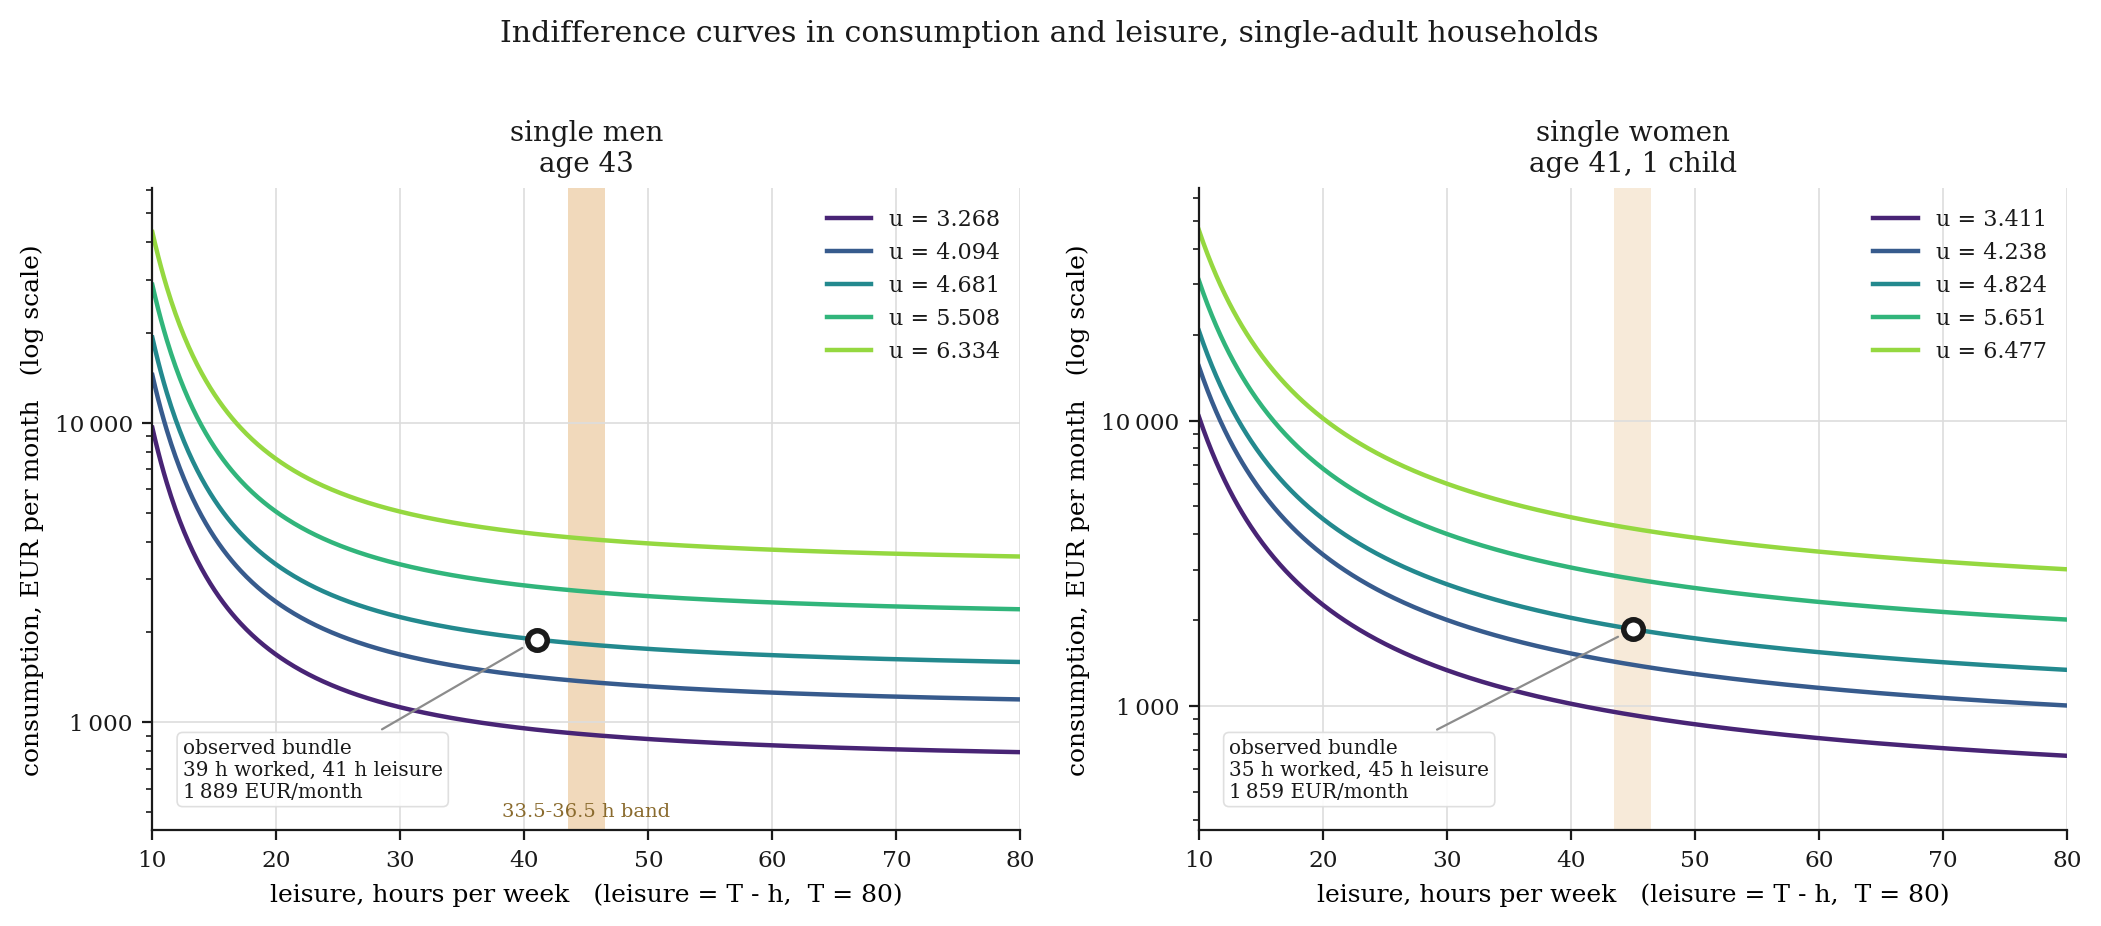
\includegraphics[width=0.95\linewidth,height=\textheight,keepaspectratio,alt={Indifference curves in consumption and leisure, single-adult households, at one representative household of each sex. The budget set, the opportunity density and the taste shock are not drawn, so a curve is not a set of attainable bundles. The consumption axis is logarithmic; under log consumption every finite utility target is attainable at a finite positive consumption, which may lie outside the plotted range.}]{figures/v5/figP01_indifference_curves_singles.png}
\caption{Indifference curves in consumption and leisure, single-adult households, at one representative household of each sex. The budget set, the opportunity density and the taste shock are not drawn, so a curve is not a set of attainable bundles. The consumption axis is logarithmic; under log consumption every finite utility target is attainable at a finite positive consumption, which may lie outside the plotted range.}
\end{figure}

\begin{figure}[H]
\centering
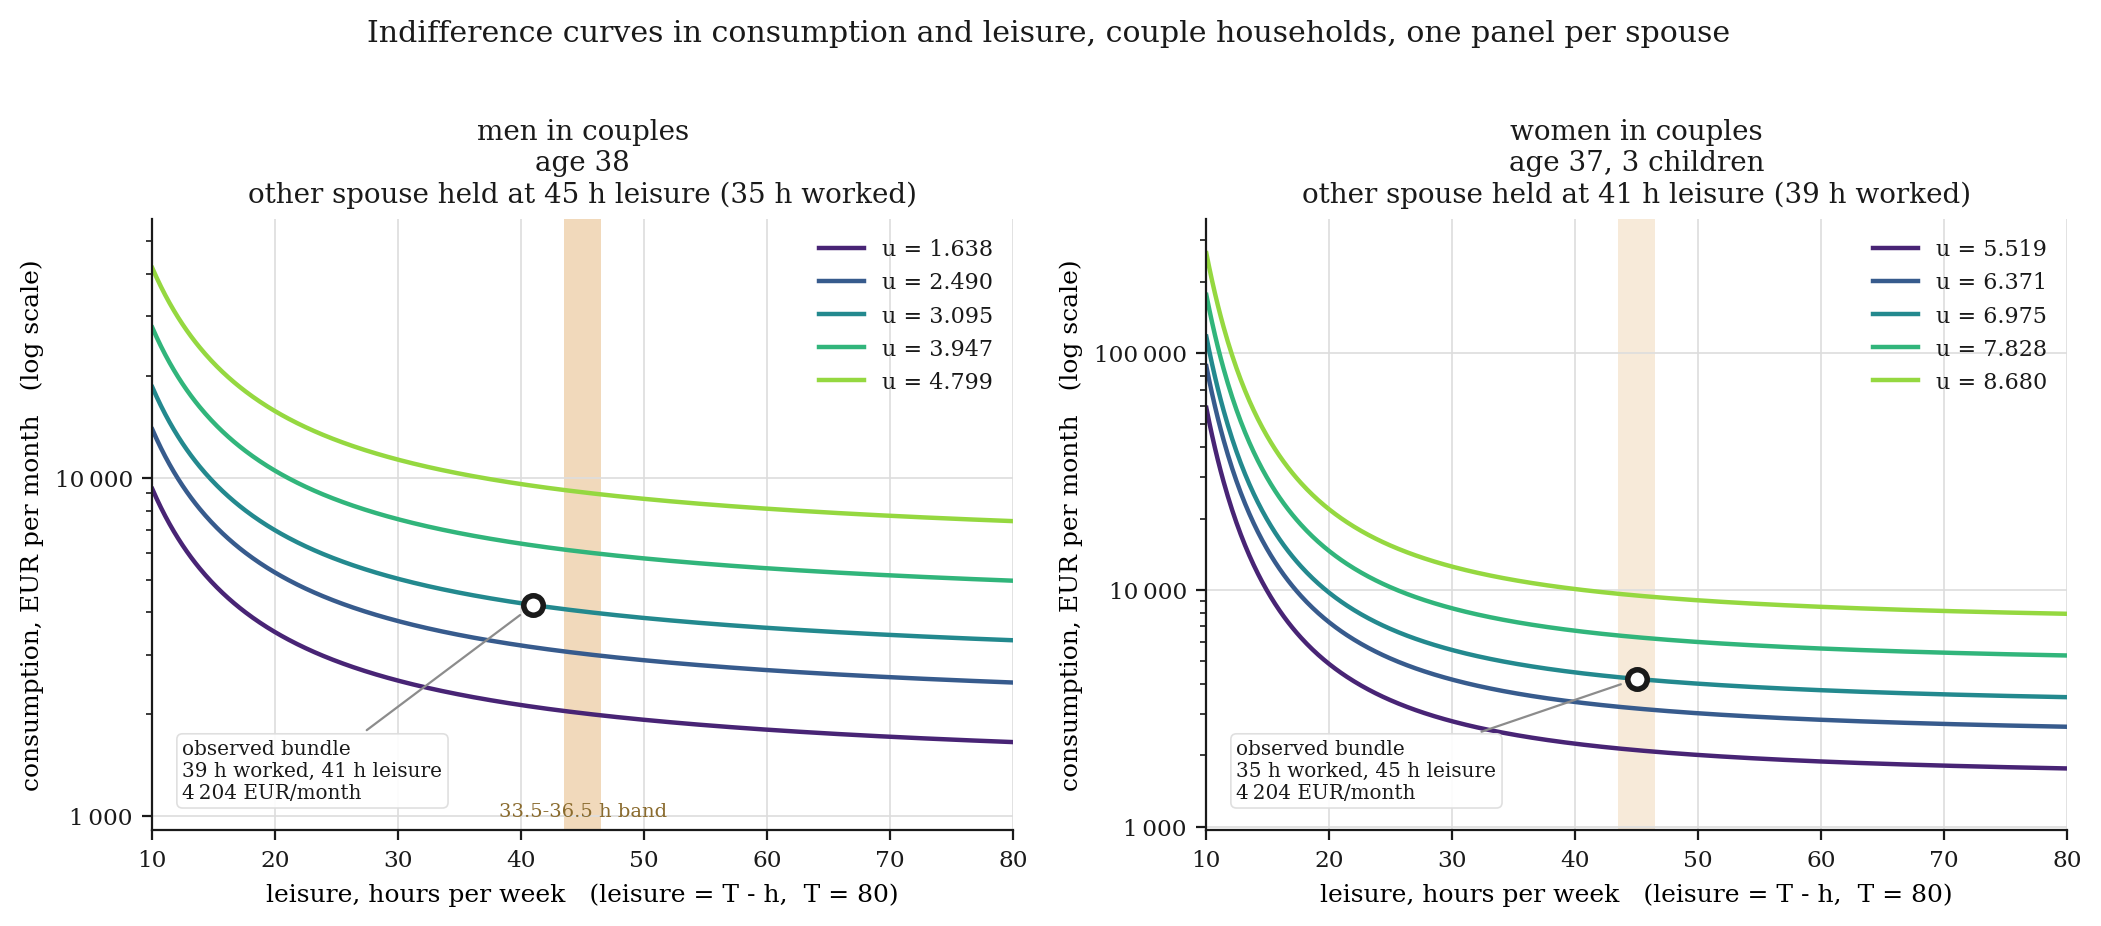
\includegraphics[width=0.95\linewidth,height=\textheight,keepaspectratio,alt={Indifference curves in consumption and each spouse's leisure, couple households, with the partner's leisure held at its observed value. Conditional slices of a joint object, not attainable sets.}]{figures/v5/figP02_indifference_curves_couples.png}
\caption{Indifference curves in consumption and each spouse's leisure, couple households, with the partner's leisure held at its observed value. Conditional slices of a joint object, not attainable sets.}
\end{figure}

\begin{figure}[H]
\centering
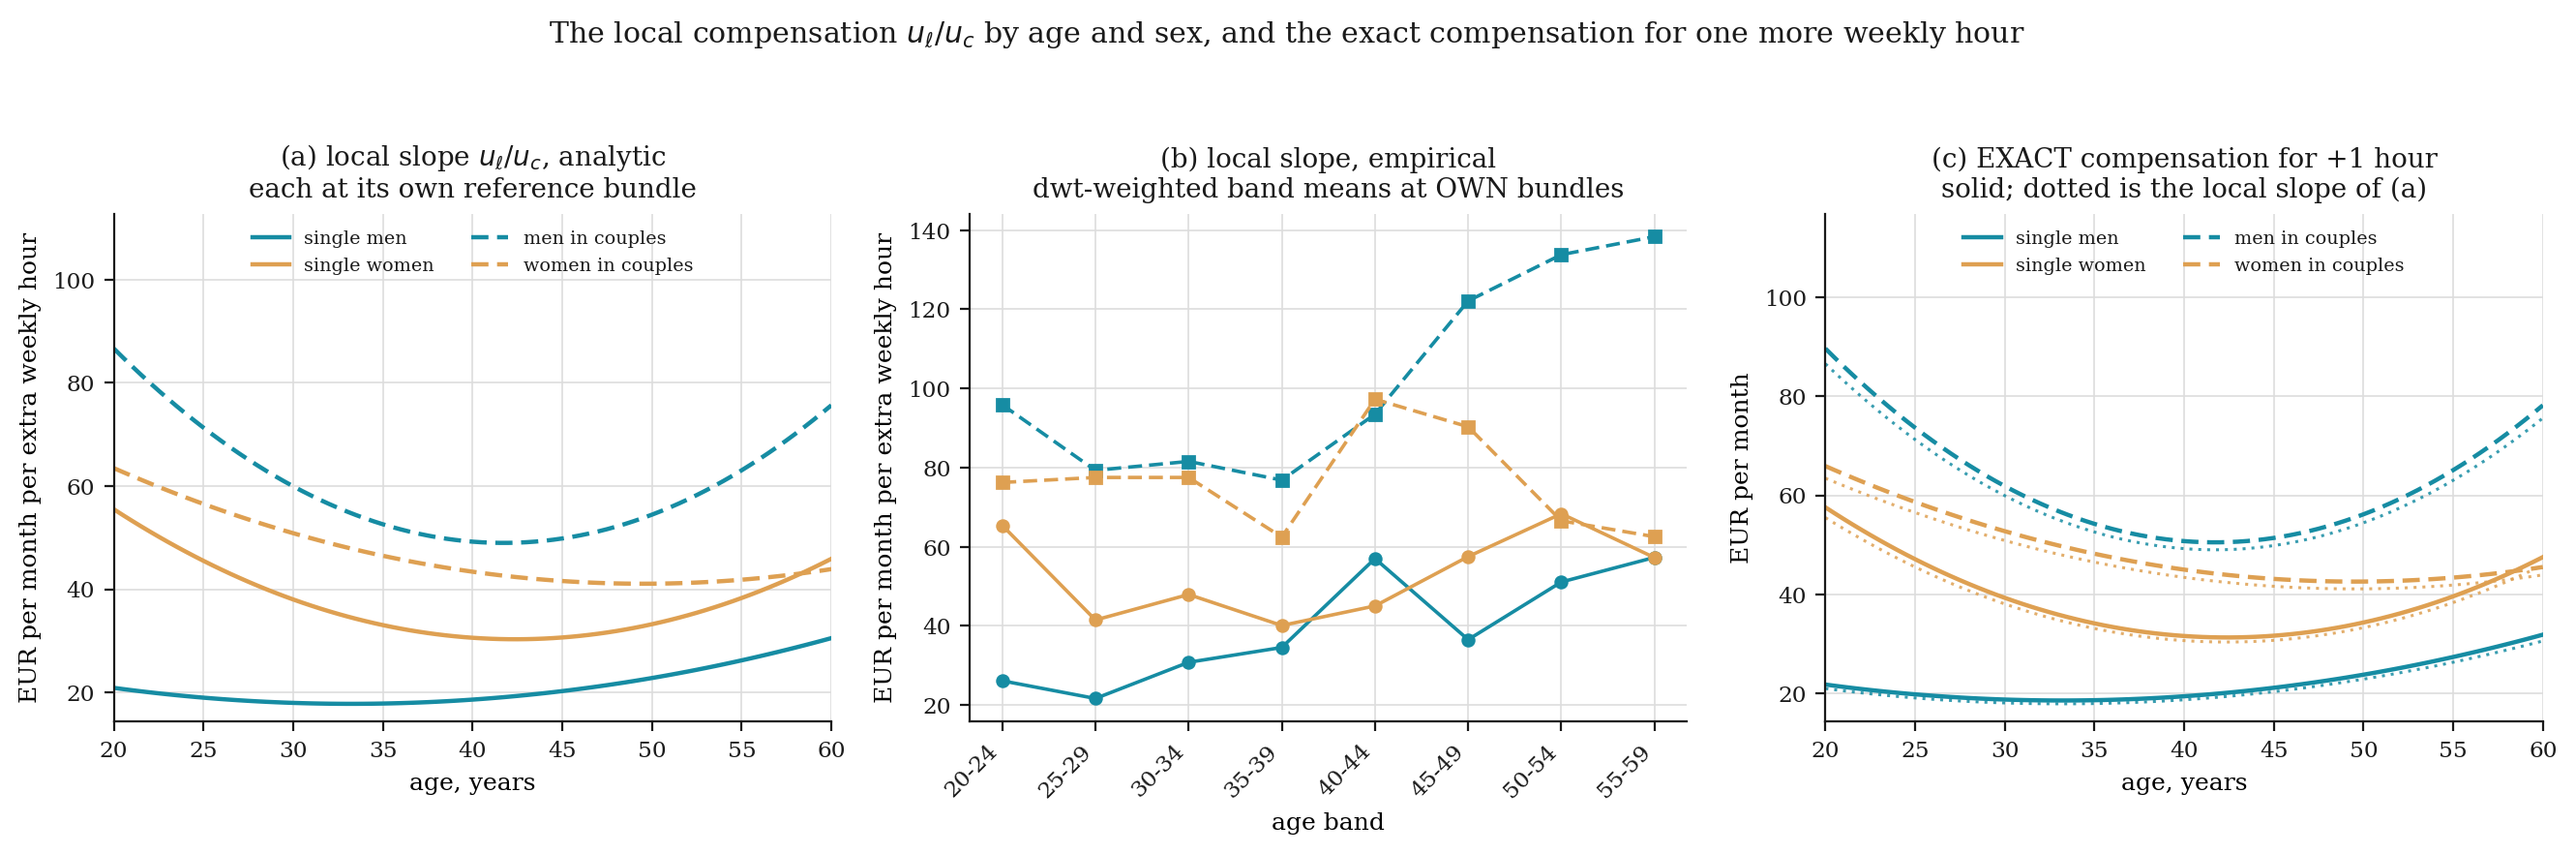
\includegraphics[width=0.95\linewidth,height=\textheight,keepaspectratio,alt={Marginal rate of substitution between leisure and consumption, by age and sex, in euros per month per additional recurring weekly hour of leisure. A compensation along an indifference curve, not a behavioural response to a wage change.}]{figures/v5/figP04_mrs_by_age_sex.png}
\caption{Marginal rate of substitution between leisure and consumption, by age and sex, in euros per month per additional recurring weekly hour of leisure. A compensation along an indifference curve, not a behavioural response to a wage change.}
\end{figure}

The indifference curves and the marginal rate of substitution are the economics; the coefficients are coordinates. Note that the consumption axis is logarithmic and the curves are drawn over the plotted range only: under \(L(\ell)+\beta_c\log(C/\lambda_c)\), any finite utility target at positive leisure is reached at the finite positive consumption \(C=\lambda_c\exp\{(\bar u-L(\ell))/\beta_c\}\), which is strictly positive for every finite target. A curve leaving the frame has left the plotting range, not the domain of the model, and nothing here is economically infeasible.

\subsection{Fit}\label{fit}

The fit reported here is a population prediction, computed by integrating the estimated model over the opportunity distribution and the taste shocks. It is not a sampled-menu choice probability and it is not an in-sample fitted value. We report it band-referenced: each group's weighted extensive-margin accuracy is compared not to a 100 per cent target -- a correctly specified stochastic-choice model does not attain one -- but to the 95 per cent band that model itself would produce by chance, from 500 outcome vectors simulated at the fitted estimates.

\begin{figure}[H]
\centering
\includegraphics[width=0.95\linewidth,height=\textheight,keepaspectratio,alt={Weighted extensive-margin accuracy against the model's own simulated 95 per cent band (500 outcome vectors at the fitted estimates), restricted to groups whose statistic clears the pre-registered numerical-adequacy gate; single men do not clear it and are withheld. Observed and band values: coupled women 89.8\% {[}88.7, 91.6{]}; single women 85.5\% {[}80.8, 86.6{]}; coupled men 92.3\% {[}89.2, 92.1{]}. Source: individual-level predictive diagnostics.}]{figures/v5/fitext_band_v1.png}
\caption{Weighted extensive-margin accuracy against the model's own simulated 95 per cent band (500 outcome vectors at the fitted estimates), restricted to groups whose statistic clears the pre-registered numerical-adequacy gate; single men do not clear it and are withheld. Observed and band values: coupled women 89.8\% {[}88.7, 91.6{]}; single women 85.5\% {[}80.8, 86.6{]}; coupled men 92.3\% {[}89.2, 92.1{]}. Source: individual-level predictive diagnostics.}
\end{figure}

Aggregate participation and occupation margins are reproduced reasonably closely, while hours fit is uneven. Individual-level predictive diagnostics raise possible excess stochastic dispersion in some groups; the group-level classification is not used as a headline result.

The figure below shows each group's weighted extensive-margin accuracy against its own simulated 95 per cent band, restricted to groups whose extensive-accuracy statistic clears the pre-registered numerical-adequacy gate (Monte Carlo simulation error at most 0.25 times the same sampling variation): coupled women, coupled men and single women clear it on the weighted statistic and are shown; single men do not and are withheld rather than shown with a caveat, because a statistic the quadrature cannot resolve is not a weaker finding, it is not a finding. Coupled men clear the weighted gate only narrowly -- ratio 0.240 against the 0.25 threshold -- and miss the unweighted version, 0.250; the weighted rule is applied throughout. Among the displayed groups, observed accuracy is inside its band for coupled women and single women, and above the top of its band for coupled men. Clearing this extensive-accuracy gate is a narrower question than the group-level fit classification discussed in the limitations below, which draws on a wider set of statistics and is inconclusive -- not passing -- for single women specifically. Section 6 records where the fuller diagnostic set -- calibration by predicted decile, the joint hours/occupation confusion structure, and the group withheld here -- still has open questions.

\subsection{Within-sample equivalised results}\label{within-sample-equivalised-results}

\Needspace*{12\baselineskip}\small\setlength{\tabcolsep}{3pt}\begin{longtable}[]{@{}
  >{\raggedright\arraybackslash}p{(\linewidth - 18\tabcolsep) * \real{0.1000}}
  >{\raggedright\arraybackslash}p{(\linewidth - 18\tabcolsep) * \real{0.1000}}
  >{\raggedright\arraybackslash}p{(\linewidth - 18\tabcolsep) * \real{0.1000}}
  >{\raggedright\arraybackslash}p{(\linewidth - 18\tabcolsep) * \real{0.1000}}
  >{\raggedright\arraybackslash}p{(\linewidth - 18\tabcolsep) * \real{0.1000}}
  >{\raggedright\arraybackslash}p{(\linewidth - 18\tabcolsep) * \real{0.1000}}
  >{\raggedright\arraybackslash}p{(\linewidth - 18\tabcolsep) * \real{0.1000}}
  >{\raggedright\arraybackslash}p{(\linewidth - 18\tabcolsep) * \real{0.1000}}
  >{\raggedright\arraybackslash}p{(\linewidth - 18\tabcolsep) * \real{0.1000}}
  >{\raggedright\arraybackslash}p{(\linewidth - 18\tabcolsep) * \real{0.1000}}@{}}
\caption{The verified own-set equal-consumption \(W^1_F\) construction, modified-OECD equivalised, against equivalised disposable consumption in the same sample. Household EUR/month, dwt-weighted. The sample aggregates are reproduced to machine precision, confirmed by an independent reimplementation. Reported separately by population; no pooled figure and no cross-population level comparison.}\tabularnewline
\toprule\noalign{}
\begin{minipage}[b]{\linewidth}\raggedright
Population
\end{minipage} & \begin{minipage}[b]{\linewidth}\raggedright
N
\end{minipage} & \begin{minipage}[b]{\linewidth}\raggedright
Workers
\end{minipage} & \begin{minipage}[b]{\linewidth}\raggedright
Non-workers
\end{minipage} & \begin{minipage}[b]{\linewidth}\raggedright
\(C^{eq}\) mean
\end{minipage} & \begin{minipage}[b]{\linewidth}\raggedright
\(C^{eq}\) median
\end{minipage} & \begin{minipage}[b]{\linewidth}\raggedright
\(C^{eq}\) Gini
\end{minipage} & \begin{minipage}[b]{\linewidth}\raggedright
\(W^1_F{}^{eq}\) mean
\end{minipage} & \begin{minipage}[b]{\linewidth}\raggedright
\(W^1_F{}^{eq}\) median
\end{minipage} & \begin{minipage}[b]{\linewidth}\raggedright
\(W^1_F{}^{eq}\) Gini
\end{minipage} \\
\midrule\noalign{}
\endfirsthead
\toprule\noalign{}
\begin{minipage}[b]{\linewidth}\raggedright
Population
\end{minipage} & \begin{minipage}[b]{\linewidth}\raggedright
N
\end{minipage} & \begin{minipage}[b]{\linewidth}\raggedright
Workers
\end{minipage} & \begin{minipage}[b]{\linewidth}\raggedright
Non-workers
\end{minipage} & \begin{minipage}[b]{\linewidth}\raggedright
\(C^{eq}\) mean
\end{minipage} & \begin{minipage}[b]{\linewidth}\raggedright
\(C^{eq}\) median
\end{minipage} & \begin{minipage}[b]{\linewidth}\raggedright
\(C^{eq}\) Gini
\end{minipage} & \begin{minipage}[b]{\linewidth}\raggedright
\(W^1_F{}^{eq}\) mean
\end{minipage} & \begin{minipage}[b]{\linewidth}\raggedright
\(W^1_F{}^{eq}\) median
\end{minipage} & \begin{minipage}[b]{\linewidth}\raggedright
\(W^1_F{}^{eq}\) Gini
\end{minipage} \\
\midrule\noalign{}
\endhead
\bottomrule\noalign{}
\endlastfoot
Single-adult & 1,540 & 1,336 & 204 & 1,766 & 1,588 & 0.2633 & 1,302 & 1,165 & 0.2498 \\
Couple & 2,223 & 2,173 & 50 & 2,245 & 2,063 & 0.2268 & 1,311 & 1,237 & 0.1974 \\
\end{longtable}

The verified \(W^1_F\) construction gives, on the modified-OECD-equivalised basis, a weighted Gini of 0.2498 for single-adult households and 0.1974 for couples, against 0.2633 and 0.2268 for equivalised disposable consumption in the same samples. This is a within-sample descriptive dispersion comparison, not a welfare-loss statement: the ratio \(W^1_F/C^{\mathrm{obs}}\) reflects the systematic leisure term at the observed job relative to home leisure, and we do not construct a loss index from it. Singles and couples are reported separately throughout, with no pooled distribution and no cross-sample level comparison: the two are separate estimation frames with different welfare units, and a comparison of the two levels is not drawn here or elsewhere in this paper.

\section{Sensitivity and limitations}\label{sensitivity-and-limitations}

\subsection{Two open econometric questions}\label{two-open-econometric-questions}

The sample screens on the observed hours and wage of employed deciders. The estimation sample is therefore selected on an outcome of the process being modelled, and the conditional sampled-set likelihood, which is the right object given a sampled choice set, is not automatically the right object given an outcome-selected sample. We have not established which correction the screen requires, or that none is required. This is an econometric question and not a presentational one, and it is not resolved by the diagnostics reported above.

Separately, the sampled-set probability is derived by conditioning on a labelled collection of slots. Small observed cross-coordinate correlations and a multiplicity distribution consistent with independent draws are diagnostics; they do not by themselves establish the sampling law that the derivation assumes. Both questions are recorded here as open.

\subsection{Limitations}\label{limitations}

The limitations travel with the results above, named together here rather than scattered through the text they qualify.

\textbf{Single men's extensive-accuracy statistic is quadrature-limited.} It fails the pre-registered numerical-adequacy gate and is withheld rather than reported at all (Section 5); the raw employment rate is matched closely (1.3 percentage points), but on the margin where this group's fit is worst, the near-full-time hours band, the record specification under-predicts by 9.5 percentage points, the largest single discrepancy in either sample. This is a genuine, group-specific fit limitation, not a tail-coverage artefact of the kind reported for the sub-ten-hour cell.

\textbf{Wage elasticities are omitted.} A valid gross-wage perturbation requires new tax-benefit repricing over the affected job alternatives, and the current priced support does not contain that counterfactual. No approximate or mock elasticity figure is reported.

\textbf{The time endowment, \(T=80\) hours a week, is a convention the model is not indifferent to.} A diagnostic re-estimation at \(T=75\) and \(T=90\), holding the rest of the certified protocol fixed, moves the criterion materially in both directions and changes which coordinates are interior: at \(T=90\) a second leisure-curvature coefficient joins the boundary that is interior at \(T=80\). \(T=80\) is therefore a maintained convention, not a free normalization the results are invariant to, and it has not itself been estimated or justified.

\textbf{Individual-level predictive diagnostics raise possible excess stochastic dispersion in some groups; the group-level classification is not used as a headline result.} The pre-registered composite decision rule flags couples (both sexes) and single men, on the weighted statistics, with a misspecification-evidence verdict against the model's own simulated variation, rather than a mechanical consequence of conditioning on outcomes. Single women's verdict is inconclusive, but not because they fail the extensive-margin numerical-adequacy gate reported above -- they clear that gate on both weighted and unweighted statistics. Their inconclusive verdict traces instead to a different set of statistics (the prediction-conditioned regression-to-the-mean check and several hard-classification and reliability statistics) failing their own, separately applied adequacy gate. Two of the four group verdicts are themselves sensitive to the weighting convention -- coupled men's underlying gate status and single men's misspecification verdict do not survive switching from weighted to unweighted statistics. This is diagnostic evidence from a composite decision rule, not a single statistic, it is sensitive to unsupported finite-panel regions being floored rather than excluded, and the underlying verdicts remain open pending further review; we report it as an open question about the model's implied stochasticity, not as an established fact about it.

\subsection{What is not established}\label{what-is-not-established}

The preliminary decomposition is an accounting of a structural model under declared operators. It is not a causal analysis. No regional, educational or occupational effect reported here is identified as a causal effect, and the exhaustiveness of the allocation validates the accounting for the declared game, not the identification of the model or the normative content of the operators.

\section{Conclusion}\label{conclusion}

Observed hours and earnings do not say whether a household chose its position or settled for it, and that ambiguity is not a nuisance for welfare measurement: it is the substance of it. This paper takes the ambiguity seriously in both halves of the problem. On the behavioural side, preferences and opportunity components are jointly estimated, with their separation relying on maintained functional-form and exclusion restrictions; every alternative is priced through the tax-benefit system. On the normative side, the money metric is derived from the own-set equal-consumption principle. Under the current empirical specification its direct reference collapses to the universally available non-employment state; opportunity heterogeneity therefore affects the current welfare measure through attained bundles.

The observed-bundle welfare and resource distributions are the descriptive welfare results. Appendix D preserves the computed preliminary restricted-operator decomposition and states its scope; it does not identify a comprehensive contribution of unequal opportunities to inequality.

\appendix

\section{Appendix A. The estimated parameter vectors}\label{appendix-a.-the-estimated-parameter-vectors}

The tables below report only coordinates estimated on the reported sample. \textbf{Maintained restrictions.} Singles: \texttt{theta\_c\_singles\ =\ 0}; the couples preference block (\texttt{beta\_l0\_m}, \texttt{beta\_l\_age\_m}, \texttt{beta\_l\_age2\_m}, \texttt{beta\_l0\_f}, \texttt{beta\_l\_age\_f}, \texttt{beta\_l\_age2\_f}, \texttt{beta\_l\_nkids\_f}, \texttt{theta\_l\_f}) does not enter the singles likelihood; and \texttt{beta\_E\_y2015} and \texttt{beta\_E\_y2017} are absent because the 2015 and 2017 data are not used. Couples: \texttt{theta\_c\ =\ 0}, the male children leisure effect is structurally zero, and the direct cross-leisure term is fixed at zero. These are restrictions, not estimates.

One single-adult coordinate, the female age-square term, is at its box endpoint. Under the active-set convention its interval is not reported, the interior curvature is computed after removing it, and the parameter draws used for the welfare intervals hold it at its estimate.

\Needspace*{12\baselineskip}\small\setlength{\tabcolsep}{3pt}\begin{longtable}[]{@{}>{\RaggedRight\arraybackslash}p{0.2500\linewidth}>{\RaggedRight\arraybackslash}p{0.1292\linewidth}>{\RaggedRight\arraybackslash}p{0.1292\linewidth}>{\RaggedRight\arraybackslash}p{0.1292\linewidth}>{\RaggedRight\arraybackslash}p{0.1292\linewidth}>{\RaggedRight\arraybackslash}p{0.1292\linewidth}@{}}
\caption{The singles estimated coordinates. Standard errors are cluster-robust on the household; boundary-active estimates are marked at bound. Maintained restrictions are stated once in the accompanying note.}\tabularnewline
\toprule\noalign{}
Coordinate & Estimate & CR1 s.e. & z & Box & Status \\
\midrule\noalign{}
\endfirsthead
\toprule\noalign{}
Coordinate & Estimate & CR1 s.e. & z & Box & Status \\
\midrule\noalign{}
\endhead
\bottomrule\noalign{}
\endlastfoot
\path{beta_l0_sm} & 8.51993 & 3.54798 & 2.401 & {[}0.05, 50{]} & estimated \\
\path{beta_l_age_sm} & 1.48195 & 1.02361 & 1.448 & {[}-5, 5{]} & estimated \\
\path{beta_l_age2_sm} & 0.778284 & 0.773158 & 1.007 & {[}-1, 1{]} & estimated \\
\path{theta_l_sm} & -1.62627 & 0.330058 & -4.927 & {[}-8, 0.95{]} & estimated \\
\path{beta_l0_sf} & 5.86829 & 2.13459 & 2.749 & {[}0.05, 50{]} & estimated \\
\path{beta_l_age_sf} & 0.0677662 & 0.479217 & 0.141 & {[}-5, 5{]} & estimated \\
\path{beta_l_age2_sf} & 1 & -- & -- & {[}-1, 1{]} & at bound \\
\path{beta_l_nkids_sf} & 0.166636 & 0.442236 & 0.377 & {[}-5, 5{]} & estimated \\
\path{theta_l_sf} & -0.927353 & 0.216128 & -4.291 & {[}-8, 0.95{]} & estimated \\
\path{beta_E} & -3.17353 & 0.405337 & -7.829 & {[}-25, 25{]} & estimated \\
\path{beta_h_pt1} & 0.0297672 & 0.197247 & 0.151 & {[}-10, 10{]} & estimated \\
\path{beta_h_pt2} & 0.707971 & 0.192788 & 3.672 & {[}-10, 10{]} & estimated \\
\path{beta_h_ft} & 1.93873 & 0.0996968 & 19.446 & {[}-10, 10{]} & estimated \\
\path{beta_h_lh} & -0.0833752 & 0.177201 & -0.471 & {[}-10, 10{]} & estimated \\
\path{beta_E_gsur} & -1.44224 & 0.235591 & -6.122 & {[}-10, 10{]} & estimated \\
\path{beta_E_drgn2} & -0.377963 & 0.32925 & -1.148 & {[}-10, 10{]} & estimated \\
\path{beta_E_drgn3} & -0.111713 & 0.38912 & -0.287 & {[}-10, 10{]} & estimated \\
\path{beta_E_drgn4} & -0.821813 & 0.380963 & -2.157 & {[}-10, 10{]} & estimated \\
\path{beta_E_drgn5} & -0.516158 & 0.327362 & -1.577 & {[}-10, 10{]} & estimated \\
\path{beta_E_drgn6} & -0.722159 & 0.35278 & -2.047 & {[}-10, 10{]} & estimated \\
\path{beta_E_drgn7} & -0.537369 & 0.350308 & -1.534 & {[}-10, 10{]} & estimated \\
\path{beta_E_drgn8} & -0.45119 & 0.340074 & -1.327 & {[}-10, 10{]} & estimated \\
\path{beta_E_drgur} & -0.0287689 & 0.220916 & -0.130 & {[}-10, 10{]} & estimated \\
\path{beta_E_drgmd} & 0.064133 & 0.261352 & 0.245 & {[}-10, 10{]} & estimated \\
\path{beta_occ_2_m} & -1.37371 & 0.158147 & -8.686 & {[}-15, 15{]} & estimated \\
\path{beta_occ_3_m} & -2.10963 & 0.202248 & -10.431 & {[}-15, 15{]} & estimated \\
\path{beta_occ_4_m} & -0.325897 & 0.121341 & -2.686 & {[}-15, 15{]} & estimated \\
\path{beta_occ_2_f} & 0.113492 & 0.137399 & 0.826 & {[}-15, 15{]} & estimated \\
\path{beta_occ_3_f} & -0.406009 & 0.144045 & -2.819 & {[}-15, 15{]} & estimated \\
\path{beta_occ_4_f} & 0.563216 & 0.122467 & 4.599 & {[}-15, 15{]} & estimated \\
\path{beta_w0} & 2.01382 & 0.0560922 & 35.902 & {[}-10, 20{]} & estimated \\
\path{beta_w_educL} & 0.0566261 & 0.0372485 & 1.520 & {[}-5, 5{]} & estimated \\
\path{beta_w_educH} & 0.149054 & 0.0308408 & 4.833 & {[}-5, 5{]} & estimated \\
\path{beta_w_pexp} & 0.24077 & 0.0862223 & 2.792 & {[}-1, 1{]} & estimated \\
\path{beta_w_pexp2} & -0.0281739 & 0.0389905 & -0.723 & {[}-0.1, 0.1{]} & estimated \\
\path{sigma} & 0.381505 & 0.0132752 & 28.738 & {[}0.1, 20{]} & estimated \\
\path{delta_occ_2} & -0.0347155 & 0.039899 & -0.870 & {[}-4, 4{]} & estimated \\
\path{delta_occ_3} & 0.0622139 & 0.0382749 & 1.625 & {[}-4, 4{]} & estimated \\
\path{delta_occ_4} & 0.278494 & 0.0367705 & 7.574 & {[}-4, 4{]} & estimated \\
\path{beta_h_f35} & 2.06556 & 0.0894479 & 23.092 & {[}-10, 10{]} & estimated \\
\path{beta_c} & 2.03873 & 0.291729 & 6.988 & {[}0.05, 50{]} & estimated \\
\end{longtable}

\Needspace*{12\baselineskip}\small\setlength{\tabcolsep}{3pt}\begin{longtable}[]{@{}>{\RaggedRight\arraybackslash}p{0.2500\linewidth}>{\RaggedRight\arraybackslash}p{0.1292\linewidth}>{\RaggedRight\arraybackslash}p{0.1292\linewidth}>{\RaggedRight\arraybackslash}p{0.1292\linewidth}>{\RaggedRight\arraybackslash}p{0.1292\linewidth}>{\RaggedRight\arraybackslash}p{0.1292\linewidth}@{}}
\caption{The couples estimated coordinates. Standard errors are cluster-robust on the household; boundary-active estimates are marked at bound. Maintained restrictions are stated once in the accompanying note.}\tabularnewline
\toprule\noalign{}
Coordinate & Estimate & CR1 s.e. & z & Box & Status \\
\midrule\noalign{}
\endfirsthead
\toprule\noalign{}
Coordinate & Estimate & CR1 s.e. & z & Box & Status \\
\midrule\noalign{}
\endhead
\bottomrule\noalign{}
\endlastfoot
\path{beta_l0_m} & 3.98136 & 0.746569 & 5.333 & {[}1e-06, 50{]} & estimated \\
\path{beta_l_age_m} & -0.00799228 & 0.0287174 & -0.278 & {[}-5, 5{]} & estimated \\
\path{beta_l_age2_m} & 0.00648336 & 0.00297388 & 2.180 & {[}-1, 1{]} & estimated \\
\path{theta_l_m} & -0.976109 & 0.135663 & -7.195 & {[}-8, 0.95{]} & estimated \\
\path{beta_l0_f} & 13.1029 & 4.77604 & 2.743 & {[}0.05, 50{]} & estimated \\
\path{beta_l_age_f} & -0.122813 & 0.126048 & -0.974 & {[}-5, 5{]} & estimated \\
\path{beta_l_age2_f} & 0.00730709 & 0.0102503 & 0.713 & {[}-1, 1{]} & estimated \\
\path{beta_l_nkids_f} & -0.305471 & 1.14719 & -0.266 & {[}-5, 5{]} & estimated \\
\path{theta_l_f} & -1.68631 & 0.245846 & -6.859 & {[}-8, 0.95{]} & estimated \\
\path{beta_E_m} & -2.12326 & 0.319457 & -6.646 & {[}-25, 25{]} & estimated \\
\path{beta_E_f} & -2.81476 & 0.302078 & -9.318 & {[}-25, 25{]} & estimated \\
\path{beta_h_pt1_m} & -1.10936 & 0.379086 & -2.926 & {[}-10, 10{]} & estimated \\
\path{beta_h_pt1_f} & -0.517276 & 0.162932 & -3.175 & {[}-10, 10{]} & estimated \\
\path{beta_h_pt2_m} & 0.0835202 & 0.237788 & 0.351 & {[}-10, 10{]} & estimated \\
\path{beta_h_pt2_f} & 1.15858 & 0.121438 & 9.541 & {[}-10, 10{]} & estimated \\
\path{beta_h_f35_m} & 2.2888 & 0.0821348 & 27.866 & {[}-10, 10{]} & estimated \\
\path{beta_h_f35_f} & 2.02835 & 0.0682392 & 29.724 & {[}-10, 10{]} & estimated \\
\path{beta_h_ft_m} & 2.38012 & 0.0865569 & 27.498 & {[}-10, 10{]} & estimated \\
\path{beta_h_ft_f} & 1.68251 & 0.0798241 & 21.078 & {[}-10, 10{]} & estimated \\
\path{beta_h_lh_m} & 0.69767 & 0.133487 & 5.226 & {[}-10, 10{]} & estimated \\
\path{beta_h_lh_f} & -0.310873 & 0.161533 & -1.925 & {[}-10, 10{]} & estimated \\
\path{beta_E_gsur} & -1.19243 & 0.155667 & -7.660 & {[}-10, 10{]} & estimated \\
\path{beta_E_drgn2} & -0.154617 & 0.24423 & -0.633 & {[}-10, 10{]} & estimated \\
\path{beta_E_drgn3} & 0.0872501 & 0.280833 & 0.311 & {[}-10, 10{]} & estimated \\
\path{beta_E_drgn4} & 0.0150136 & 0.306753 & 0.049 & {[}-10, 10{]} & estimated \\
\path{beta_E_drgn5} & -0.145472 & 0.255453 & -0.569 & {[}-10, 10{]} & estimated \\
\path{beta_E_drgn6} & -0.284391 & 0.274814 & -1.035 & {[}-10, 10{]} & estimated \\
\path{beta_E_drgn7} & -0.139569 & 0.265133 & -0.526 & {[}-10, 10{]} & estimated \\
\path{beta_E_drgn8} & -0.165927 & 0.26603 & -0.624 & {[}-10, 10{]} & estimated \\
\path{beta_E_drgur} & -0.182322 & 0.165665 & -1.101 & {[}-10, 10{]} & estimated \\
\path{beta_E_drgmd} & -0.417356 & 0.1861 & -2.243 & {[}-10, 10{]} & estimated \\
\path{beta_occ_2_m} & -1.50975 & 0.0967347 & -15.607 & {[}-15, 15{]} & estimated \\
\path{beta_occ_3_m} & -2.25319 & 0.124405 & -18.112 & {[}-15, 15{]} & estimated \\
\path{beta_occ_4_m} & 0.159368 & 0.061796 & 2.579 & {[}-15, 15{]} & estimated \\
\path{beta_occ_2_f} & 0.207379 & 0.0891054 & 2.327 & {[}-15, 15{]} & estimated \\
\path{beta_occ_3_f} & -0.180381 & 0.0923137 & -1.954 & {[}-15, 15{]} & estimated \\
\path{beta_occ_4_f} & 0.81589 & 0.079925 & 10.208 & {[}-15, 15{]} & estimated \\
\path{beta_w0} & 2.048 & 0.0335421 & 61.058 & {[}-10, 20{]} & estimated \\
\path{beta_w_educL} & -0.0433046 & 0.0216643 & -1.999 & {[}-5, 5{]} & estimated \\
\path{beta_w_educH} & 0.181652 & 0.0197059 & 9.218 & {[}-5, 5{]} & estimated \\
\path{beta_w_pexp} & 0.56435 & 0.0545928 & 10.337 & {[}-3, 3{]} & estimated \\
\path{beta_w_pexp2} & -0.15983 & 0.0242888 & -6.580 & {[}-0.3, 0.3{]} & estimated \\
\path{sigma} & 0.363075 & 0.0072235 & 50.263 & {[}0.1, 20{]} & estimated \\
\path{delta_occ_2} & -0.0740322 & 0.0231318 & -3.200 & {[}-4, 4{]} & estimated \\
\path{delta_occ_3} & 0.0393566 & 0.0228 & 1.726 & {[}-4, 4{]} & estimated \\
\path{delta_occ_4} & 0.214559 & 0.0223344 & 9.607 & {[}-4, 4{]} & estimated \\
\path{beta_c} & 2.10172 & 0.293879 & 7.152 & {[}0.05, 50{]} & estimated \\
\end{longtable}

\section{Appendix B. Inequality indices and the allocation rule}\label{appendix-b.-inequality-indices-and-the-allocation-rule}

The preliminary decomposition in Appendix D uses the Gini index only, on a weighted distribution of strictly positive money-metric levels with mean \(\mu\): \(\mathcal I=\frac{1}{2\mu}\,\mathbb{E}\lvert W-\tilde W\rvert\), for \(W,\tilde W\) independent draws from the distribution. Extending the exercise to further indices is future work and is not reported here.

The exact Shapley value on the three-player game \(v(S)=I_\varnothing-I_S\), \(S\subseteq\{P,A,B\}\), allocates to factor \(k\) the average of its marginal contribution \(v(S\cup\{k\})-v(S)\) over all \(3!=6\) orderings in which the three factors can be introduced:

\[
C_k=\frac{1}{6}\sum_{\pi}\big[v(S_\pi(k)\cup\{k\})-v(S_\pi(k))\big],
\]

where \(S_\pi(k)\) is the set of factors preceding \(k\) in ordering \(\pi\). With three players this has a closed form and requires no grouping into unions. Contributions are signed and are never renormalised to sum to one hundred by construction: they sum to \(\Delta I=I_\varnothing-I_{\{P,A,B\}}\) because the game closes, and the closure is verified.

\section{Appendix C. Data, software and replication}\label{appendix-c.-data-software-and-replication}

\textbf{Data.} French EU-SILC, accessed through Eurostat's harmonised release, with 2016 survey collection and a 2015 income reference year. The harmonised survey is transformed into an input file for EUROMOD \citep{sutherlandfigari2013}, which applies the French 2015 policy system. Regional labour-market conditions come from the Eurostat regional labour-force series. Access to EU-SILC microdata is granted by Eurostat under its research-access conditions and the data cannot be redistributed with this document.

\textbf{Sample.} 1,540 single-adult and 2,223 couple households, constructed by the screens of Section 2.

\textbf{Estimator and inference.} Conditional likelihood over 100 sampled alternatives per household plus the observed choice, with an out-of-fold proposal correction; cluster-robust standard errors on the household. Optimization is checked by five starts under two polishing contracts and curvature by exact Hessian eigenvalues.

\textbf{Welfare computation.} The verified own-set equal-consumption welfare baseline is reported from its aggregate evidence. This bounded decomposition exercise recomputes all eight coalitions in the three-player game for each reporting scale. Its uncertainty display is a Monte Carlo range across 1,000 simulation replications plus an independent second-seed check; it is not a parameter-uncertainty interval.

\textbf{Software.} Python with JAX (0.10.1) for automatic differentiation, and the EUROMOD connector (0.2.17).

\textbf{Replication.} Code and derived, non-confidential intermediate artefacts will be made available in a public replication archive on publication. Confidential microdata remain in their permitted environment, so the replication package reproduces every step conditional on authorised access to EU-SILC.

\section{Appendix D. Preliminary restricted-operator decomposition}\label{appendix-d.-preliminary-restricted-operator-decomposition}

A preliminary P/A/B decomposition has been computed for the attained-bundle money metric, holding resources, needs and composition fixed. It is a restricted counterfactual exercise, not a comprehensive share of inequality due to all opportunities. A separately defined ex-ante metric is being reconstructed for comparison; neither historical ex-ante percentages nor a settled cross-estimand conclusion are reported here.

The earning-opportunity channel equalises wage-offer location only: the systematic differences associated with education and potential experience, which shift offer locations by at most about 0.10 log points. The common offer spread (about 0.37 log points), wage-draw luck and selection remain in the residual and are quantitatively larger than the location differences removed by this operator. This is a definitional boundary of the exercise, not a measurement error. Equalising locations can change attained wages; it does not equalise the whole wage distribution. The diagnostic comparison that also compresses the common spread and selection is a bound, not an additional decomposition result. Thin effective support for couples leaves individual wage attainment noisy and remains a numerical limitation.

\subsection{Counterfactual operators and simulation rule}\label{counterfactual-operators-and-simulation-rule}

A complete attribution of measured inequality to preferences and to circumstances requires a counterfactual-attainment estimand: under a counterfactual environment, which bundle does the household attain? Two candidate estimands are under design -- a realised-bundle route conditioning the behavioural latent state on the observed choice, and an ex-ante route integrating the measure over the model-implied counterfactual choice distribution -- and neither is executed here, because the inequality of expected welfare is not the expected inequality of welfare and the two routes answer different questions. Ahead of that design choice, this section reports a bounded, explicitly preliminary exercise that reuses the model's own already-priced estimation panel, with no re-estimation and no new pricing, and simulates each household's attained bundle under a counterfactual environment by carrying the household's realised draws through it directly.

Let \(X_i=(P_i,A_i,B_i)\) collect three structural inputs for household \(i\):

\begin{itemize}
\tightlist
\item
  \(P_i\) systematic utility heterogeneity: the leisure-weight covariates and the sex- or spouse-specific preference block, including the reduced-form time-constraint shifters this pathway also carries;
\item
  \(A_i\) local geographic/temporal access shifters (region, urban/rural, year): only those arguments of the employment index; personal occupation access, hours-band access, the group-unemployment measure and node-level alternative characteristics remain fixed;
\item
  \(B_i\) earning opportunities: the covariates entering the offered-wage location.
\end{itemize}

Household resources, needs and composition are held fixed throughout this exercise rather than treated as a fourth operator: they are not equalized in any coalition and no share is attributed to them. Let \(\mathcal I\) be the Gini index and \(W_i(\cdot)\) the money metric of the previous subsection, so the baseline is \(I_\varnothing=\mathcal I\{W_i(X_i)\}_{i=1}^N\). For each factor define a \textbf{structural equalization operator} \(T_P,T_A,T_B\), which replaces that factor's arguments across all households by a common reference profile and leaves the estimated coefficients in place. For a coalition \(S\subseteq\{P,A,B\}\) let \(X^S=T_S(X)\) be the state in which exactly the factors in \(S\) are equalized, and set

\[
I_S=\mathcal I\{W_i(T_S X)\}_{i=1}^{N},
\qquad
v(S)=I_\varnothing-I_S .
\]

\(v\) is a cooperative game on three players: the worth of a coalition is the inequality it removes when its factors are equalized together. \(T_S\) is a single simultaneous substitution map, not an ordered product \(\prod_{k\in S}T_k\), and an operator changes a \emph{pathway}, not every occurrence of a raw characteristic.

\Needspace*{12\baselineskip}\small\setlength{\tabcolsep}{3pt}\begin{longtable}[]{@{}
  >{\raggedright\arraybackslash}p{(\linewidth - 4\tabcolsep) * \real{0.3333}}
  >{\raggedright\arraybackslash}p{(\linewidth - 4\tabcolsep) * \real{0.3333}}
  >{\raggedright\arraybackslash}p{(\linewidth - 4\tabcolsep) * \real{0.3333}}@{}}
\caption{The three structural equalization operators of the preliminary decomposition (Section 5). Each operator replaces the arguments of one structural pathway with a common reference profile and leaves the estimated coefficients in place; it does not equalize every occurrence of a raw characteristic. Operators are applied as one simultaneous substitution map, not as an ordered product. Household resources, needs and composition are held fixed throughout this exercise -- not a fourth operator here -- pending the counterfactual-attainment estimand the paper's final decomposition architecture requires.}\tabularnewline
\toprule\noalign{}
\begin{minipage}[b]{\linewidth}\raggedright
Operator
\end{minipage} & \begin{minipage}[b]{\linewidth}\raggedright
What is replaced
\end{minipage} & \begin{minipage}[b]{\linewidth}\raggedright
What is retained
\end{minipage} \\
\midrule\noalign{}
\endfirsthead
\toprule\noalign{}
\begin{minipage}[b]{\linewidth}\raggedright
Operator
\end{minipage} & \begin{minipage}[b]{\linewidth}\raggedright
What is replaced
\end{minipage} & \begin{minipage}[b]{\linewidth}\raggedright
What is retained
\end{minipage} \\
\midrule\noalign{}
\endhead
\bottomrule\noalign{}
\endlastfoot
\(T_P\) preferences (systematic utility heterogeneity) & Singles: the arguments of the leisure weight and the complete reference-sex leisure block. Couples: the medoid spouse arguments, with own spouse coefficients retained & Access and wage pathways of the same characteristics \\
\(T_A\) local geographic/temporal access shifters & Region, urban/rural and year arguments of the employment index & Preferences, wage location, group unemployment, hours-band access, personal occupation access and node-level alternative characteristics \\
\(T_B\) earning opportunities & The arguments of the offered-wage location: education shares and experience moments, with squares recomputed rather than averaged & The estimated wage coefficients and dispersion; the preference and access pathways of the same characteristics \\
\end{longtable}

Welfare and inequality are then recomputed from the model for all eight coalitions of \(\{P,A,B\}\). There is no linearisation and no re-estimation: coefficients are held at their estimates throughout, and only the arguments move.

The interactions are allocated with the \textbf{exact Shapley value} \citep{shorrocks2013} on the three-player game \(v\): the average of each factor's marginal contribution over all orderings in which the three factors can be equalized. With three players this average has a closed form over \(3!=6\) orderings and requires no grouping. The allocation is exhaustive: the contributions sum to \(\Delta I=I_\varnothing-I_{\{P,A,B\}}\), and we report \(\Delta I\) itself rather than treat it as identically zero, because household resources, needs and composition remain in the residual \(I_{\{P,A,B\}}\) along with sex-block parameter differences and behavioural randomness.

Uncertainty is reported two ways, never merged into a confidence interval: a Monte Carlo range across 1,000 simulation replications at fixed estimates, and an independent check under a second simulation seed. Neither is a parameter-uncertainty interval; propagating the estimation covariance into this exercise is future work.

\subsection{Coalition values and signed allocation}\label{coalition-values-and-signed-allocation}

\Needspace*{12\baselineskip}\small\setlength{\tabcolsep}{3pt}\begin{longtable}[]{@{}>{\RaggedRight\arraybackslash}p{0.2500\linewidth}>{\RaggedRight\arraybackslash}p{0.1650\linewidth}>{\RaggedRight\arraybackslash}p{0.1650\linewidth}>{\RaggedRight\arraybackslash}p{0.1650\linewidth}>{\RaggedRight\arraybackslash}p{0.1650\linewidth}@{}}
\caption{Single adults, the eight P/A/B coalitions. Weighted Gini of money-metric well-being, dwt-weighted, simulated on the estimated model's already-priced estimation panel with no re-estimation and no new pricing. ``Change from actual'' is the one-factor effect of that coalition. The Monte Carlo range is the spread of the Gini level across 1,000 simulation replications, never a confidence interval.}\tabularnewline
\toprule\noalign{}
Scale & Coalition & I(S), Gini & Change from actual & MC range (min--max) \\
\midrule\noalign{}
\endfirsthead
\toprule\noalign{}
Scale & Coalition & I(S), Gini & Change from actual & MC range (min--max) \\
\midrule\noalign{}
\endhead
\bottomrule\noalign{}
\endlastfoot
unequivalised & Actual (no equalization) & 0.2337 & +0.0000 & 0.2203--0.2509 \\
unequivalised & P & 0.2326 & -0.0011 & 0.2180--0.2491 \\
unequivalised & A & 0.2319 & -0.0018 & 0.2178--0.2480 \\
unequivalised & B & 0.2298 & -0.0039 & 0.2148--0.2452 \\
unequivalised & P + A & 0.2310 & -0.0027 & 0.2177--0.2478 \\
unequivalised & P + B & 0.2282 & -0.0054 & 0.2138--0.2437 \\
unequivalised & A + B & 0.2282 & -0.0055 & 0.2135--0.2411 \\
unequivalised & P + A + B & 0.2268 & -0.0069 & 0.2127--0.2431 \\
equivalised & Actual (no equalization) & 0.2451 & +0.0000 & 0.2284--0.2663 \\
equivalised & P & 0.2456 & +0.0005 & 0.2304--0.2647 \\
equivalised & A & 0.2436 & -0.0014 & 0.2264--0.2631 \\
equivalised & B & 0.2419 & -0.0032 & 0.2264--0.2592 \\
equivalised & P + A & 0.2443 & -0.0008 & 0.2304--0.2624 \\
equivalised & P + B & 0.2418 & -0.0033 & 0.2263--0.2594 \\
equivalised & A + B & 0.2405 & -0.0046 & 0.2245--0.2582 \\
equivalised & P + A + B & 0.2406 & -0.0045 & 0.2248--0.2580 \\
\end{longtable}

\Needspace*{12\baselineskip}\small\setlength{\tabcolsep}{3pt}\begin{longtable}[]{@{}>{\RaggedRight\arraybackslash}p{0.2500\linewidth}>{\RaggedRight\arraybackslash}p{0.1650\linewidth}>{\RaggedRight\arraybackslash}p{0.1650\linewidth}>{\RaggedRight\arraybackslash}p{0.1650\linewidth}>{\RaggedRight\arraybackslash}p{0.1650\linewidth}@{}}
\caption{Couples, the eight P/A/B coalitions. Weighted Gini of money-metric well-being, dwt-weighted, simulated on the estimated model's already-priced estimation panel with no re-estimation and no new pricing. ``Change from actual'' is the one-factor effect of that coalition. The Monte Carlo range is the spread of the Gini level across 1,000 simulation replications, never a confidence interval.}\tabularnewline
\toprule\noalign{}
Scale & Coalition & I(S), Gini & Change from actual & MC range (min--max) \\
\midrule\noalign{}
\endfirsthead
\toprule\noalign{}
Scale & Coalition & I(S), Gini & Change from actual & MC range (min--max) \\
\midrule\noalign{}
\endhead
\bottomrule\noalign{}
\endlastfoot
unequivalised & Actual (no equalization) & 0.2035 & +0.0000 & 0.1936--0.2144 \\
unequivalised & P & 0.1956 & -0.0079 & 0.1858--0.2059 \\
unequivalised & A & 0.2025 & -0.0010 & 0.1938--0.2140 \\
unequivalised & B & 0.1892 & -0.0143 & 0.1803--0.2018 \\
unequivalised & P + A & 0.1946 & -0.0089 & 0.1844--0.2046 \\
unequivalised & P + B & 0.1842 & -0.0193 & 0.1742--0.1962 \\
unequivalised & A + B & 0.1883 & -0.0152 & 0.1796--0.2000 \\
unequivalised & P + A + B & 0.1834 & -0.0201 & 0.1731--0.1944 \\
equivalised & Actual (no equalization) & 0.1971 & +0.0000 & 0.1871--0.2075 \\
equivalised & P & 0.1969 & -0.0002 & 0.1873--0.2069 \\
equivalised & A & 0.1963 & -0.0008 & 0.1869--0.2055 \\
equivalised & B & 0.1887 & -0.0084 & 0.1789--0.1998 \\
equivalised & P + A & 0.1961 & -0.0010 & 0.1861--0.2049 \\
equivalised & P + B & 0.1927 & -0.0044 & 0.1829--0.2039 \\
equivalised & A + B & 0.1880 & -0.0091 & 0.1775--0.1985 \\
equivalised & P + A + B & 0.1921 & -0.0050 & 0.1821--0.2033 \\
\end{longtable}

\begin{figure}[H]
\centering
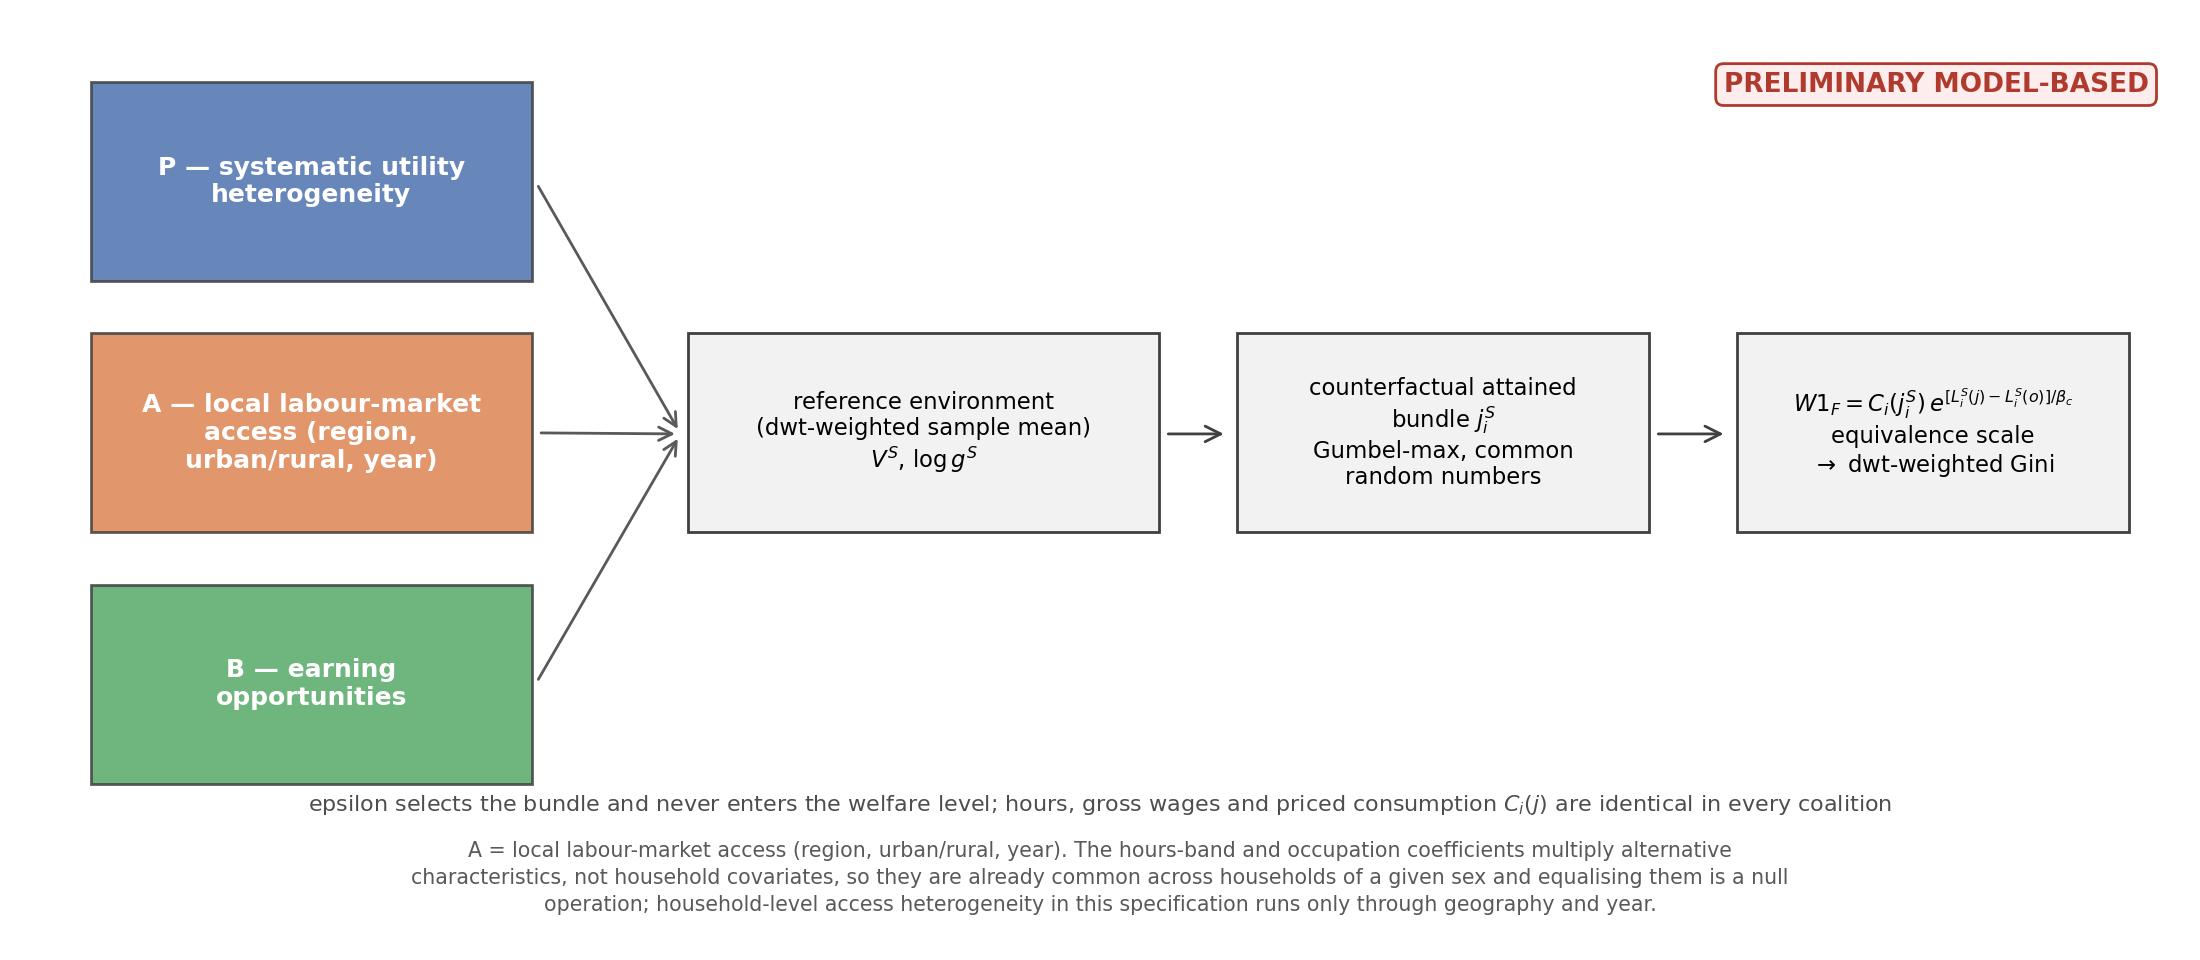
\includegraphics[width=0.95\linewidth,height=\textheight,keepaspectratio,alt={The eight P/A/B counterfactual coalitions, built from the estimated model by equalising household-constant covariates within a block. Node-level alternative characteristics are preserved in every coalition; only household-constant covariates are equalised. Preliminary, model-based.}]{figures/v5/fig_preseminar_pab_architecture_v1.png}
\caption{The eight P/A/B counterfactual coalitions, built from the estimated model by equalising household-constant covariates within a block. Node-level alternative characteristics are preserved in every coalition; only household-constant covariates are equalised. Preliminary, model-based.}
\end{figure}

The bounded percentage reported below is not evidence that opportunities are unimportant; it is the change inside the stated partial accounting game.

The decomposition is bounded by design because household resources, needs and composition are held fixed. Within that bounded game, equalising P/A/B changes the Gini by 1.8--9.9\% of its baseline level, depending on sample and reporting scale.

Dispersion in consumption is quantitatively large relative to dispersion in log well-being: \(\operatorname{Var}(\log C)\) is roughly 100--127\% of \(\operatorname{Var}(\log W)\), with the excess offset by a large negative covariance between consumption and the leisure valuation. This bounded decomposition exercise holds household resources, needs and composition fixed, leaving important sources of dispersion outside the P/A/B allocation. Sex-block parameter differences and behavioural randomness also remain in the residual and are not attributed to \(P\), \(A\) or \(B\).

\Needspace*{12\baselineskip}\small\setlength{\tabcolsep}{3pt}\begin{longtable}[]{@{}
  >{\raggedright\arraybackslash}p{(\linewidth - 12\tabcolsep) * \real{0.1429}}
  >{\raggedright\arraybackslash}p{(\linewidth - 12\tabcolsep) * \real{0.1429}}
  >{\raggedright\arraybackslash}p{(\linewidth - 12\tabcolsep) * \real{0.1429}}
  >{\raggedright\arraybackslash}p{(\linewidth - 12\tabcolsep) * \real{0.1429}}
  >{\raggedright\arraybackslash}p{(\linewidth - 12\tabcolsep) * \real{0.1429}}
  >{\raggedright\arraybackslash}p{(\linewidth - 12\tabcolsep) * \real{0.1429}}
  >{\raggedright\arraybackslash}p{(\linewidth - 12\tabcolsep) * \real{0.1429}}@{}}
\caption{The exact three-player Shapley allocation of \(\Delta I\) across P, A and B. Gini-point contribution beside the share of \(\Delta I\) (not of baseline inequality), and an independent second-seed reproduction. No directional claim is made about P: its sign changes between unequivalised and equivalised reporting in both samples, so its share of \(\Delta I\) is not stated. A Monte Carlo per-replication share range, which divides by that replication's own near-zero \(\Delta I\) and is not informative on its own, is reported in the technical gallery, not here.}\tabularnewline
\toprule\noalign{}
\begin{minipage}[b]{\linewidth}\raggedright
Population
\end{minipage} & \begin{minipage}[b]{\linewidth}\raggedright
Scale
\end{minipage} & \begin{minipage}[b]{\linewidth}\raggedright
Factor
\end{minipage} & \begin{minipage}[b]{\linewidth}\raggedright
Label
\end{minipage} & \begin{minipage}[b]{\linewidth}\raggedright
Gini-point contribution
\end{minipage} & \begin{minipage}[b]{\linewidth}\raggedright
Share of \(\Delta I\)
\end{minipage} & \begin{minipage}[b]{\linewidth}\raggedright
Second-seed Gini-point
\end{minipage} \\
\midrule\noalign{}
\endfirsthead
\toprule\noalign{}
\begin{minipage}[b]{\linewidth}\raggedright
Population
\end{minipage} & \begin{minipage}[b]{\linewidth}\raggedright
Scale
\end{minipage} & \begin{minipage}[b]{\linewidth}\raggedright
Factor
\end{minipage} & \begin{minipage}[b]{\linewidth}\raggedright
Label
\end{minipage} & \begin{minipage}[b]{\linewidth}\raggedright
Gini-point contribution
\end{minipage} & \begin{minipage}[b]{\linewidth}\raggedright
Share of \(\Delta I\)
\end{minipage} & \begin{minipage}[b]{\linewidth}\raggedright
Second-seed Gini-point
\end{minipage} \\
\midrule\noalign{}
\endhead
\bottomrule\noalign{}
\endlastfoot
Single-adult & unequivalised & P & Preferences (systematic utility heterogeneity) & +0.0012 & --- & +0.0011 \\
Single-adult & unequivalised & A & Local access shifters (region, urban/rural, year) & +0.0016 & 23.4\% & +0.0017 \\
Single-adult & unequivalised & B & Earning opportunities & +0.0040 & 58.6\% & +0.0042 \\
Single-adult & unequivalised & \(\Delta I\) & I(actual) \(-\) I(P,A,B equalized) & +0.0069 & 100.0\% & +0.0071 \\
Single-adult & equivalised & P & Preferences (systematic utility heterogeneity) & -0.0003 & --- & -0.0004 \\
Single-adult & equivalised & A & Local access shifters (region, urban/rural, year) & +0.0013 & 29.6\% & +0.0014 \\
Single-adult & equivalised & B & Earning opportunities & +0.0034 & 77.4\% & +0.0038 \\
Single-adult & equivalised & \(\Delta I\) & I(actual) \(-\) I(P,A,B equalized) & +0.0045 & 100.0\% & +0.0049 \\
Couple & unequivalised & P & Preferences (systematic utility heterogeneity) & +0.0064 & --- & +0.0065 \\
Couple & unequivalised & A & Local access shifters (region, urban/rural, year) & +0.0009 & 4.6\% & +0.0009 \\
Couple & unequivalised & B & Earning opportunities & +0.0128 & 63.5\% & +0.0127 \\
Couple & unequivalised & \(\Delta I\) & I(actual) \(-\) I(P,A,B equalized) & +0.0201 & 100.0\% & +0.0201 \\
Couple & equivalised & P & Preferences (systematic utility heterogeneity) & -0.0019 & --- & -0.0019 \\
Couple & equivalised & A & Local access shifters (region, urban/rural, year) & +0.0007 & 14.6\% & +0.0008 \\
Couple & equivalised & B & Earning opportunities & +0.0062 & 124.0\% & +0.0061 \\
Couple & equivalised & \(\Delta I\) & I(actual) \(-\) I(P,A,B equalized) & +0.0050 & 100.0\% & +0.0050 \\
\end{longtable}

\begin{figure}[H]
\centering
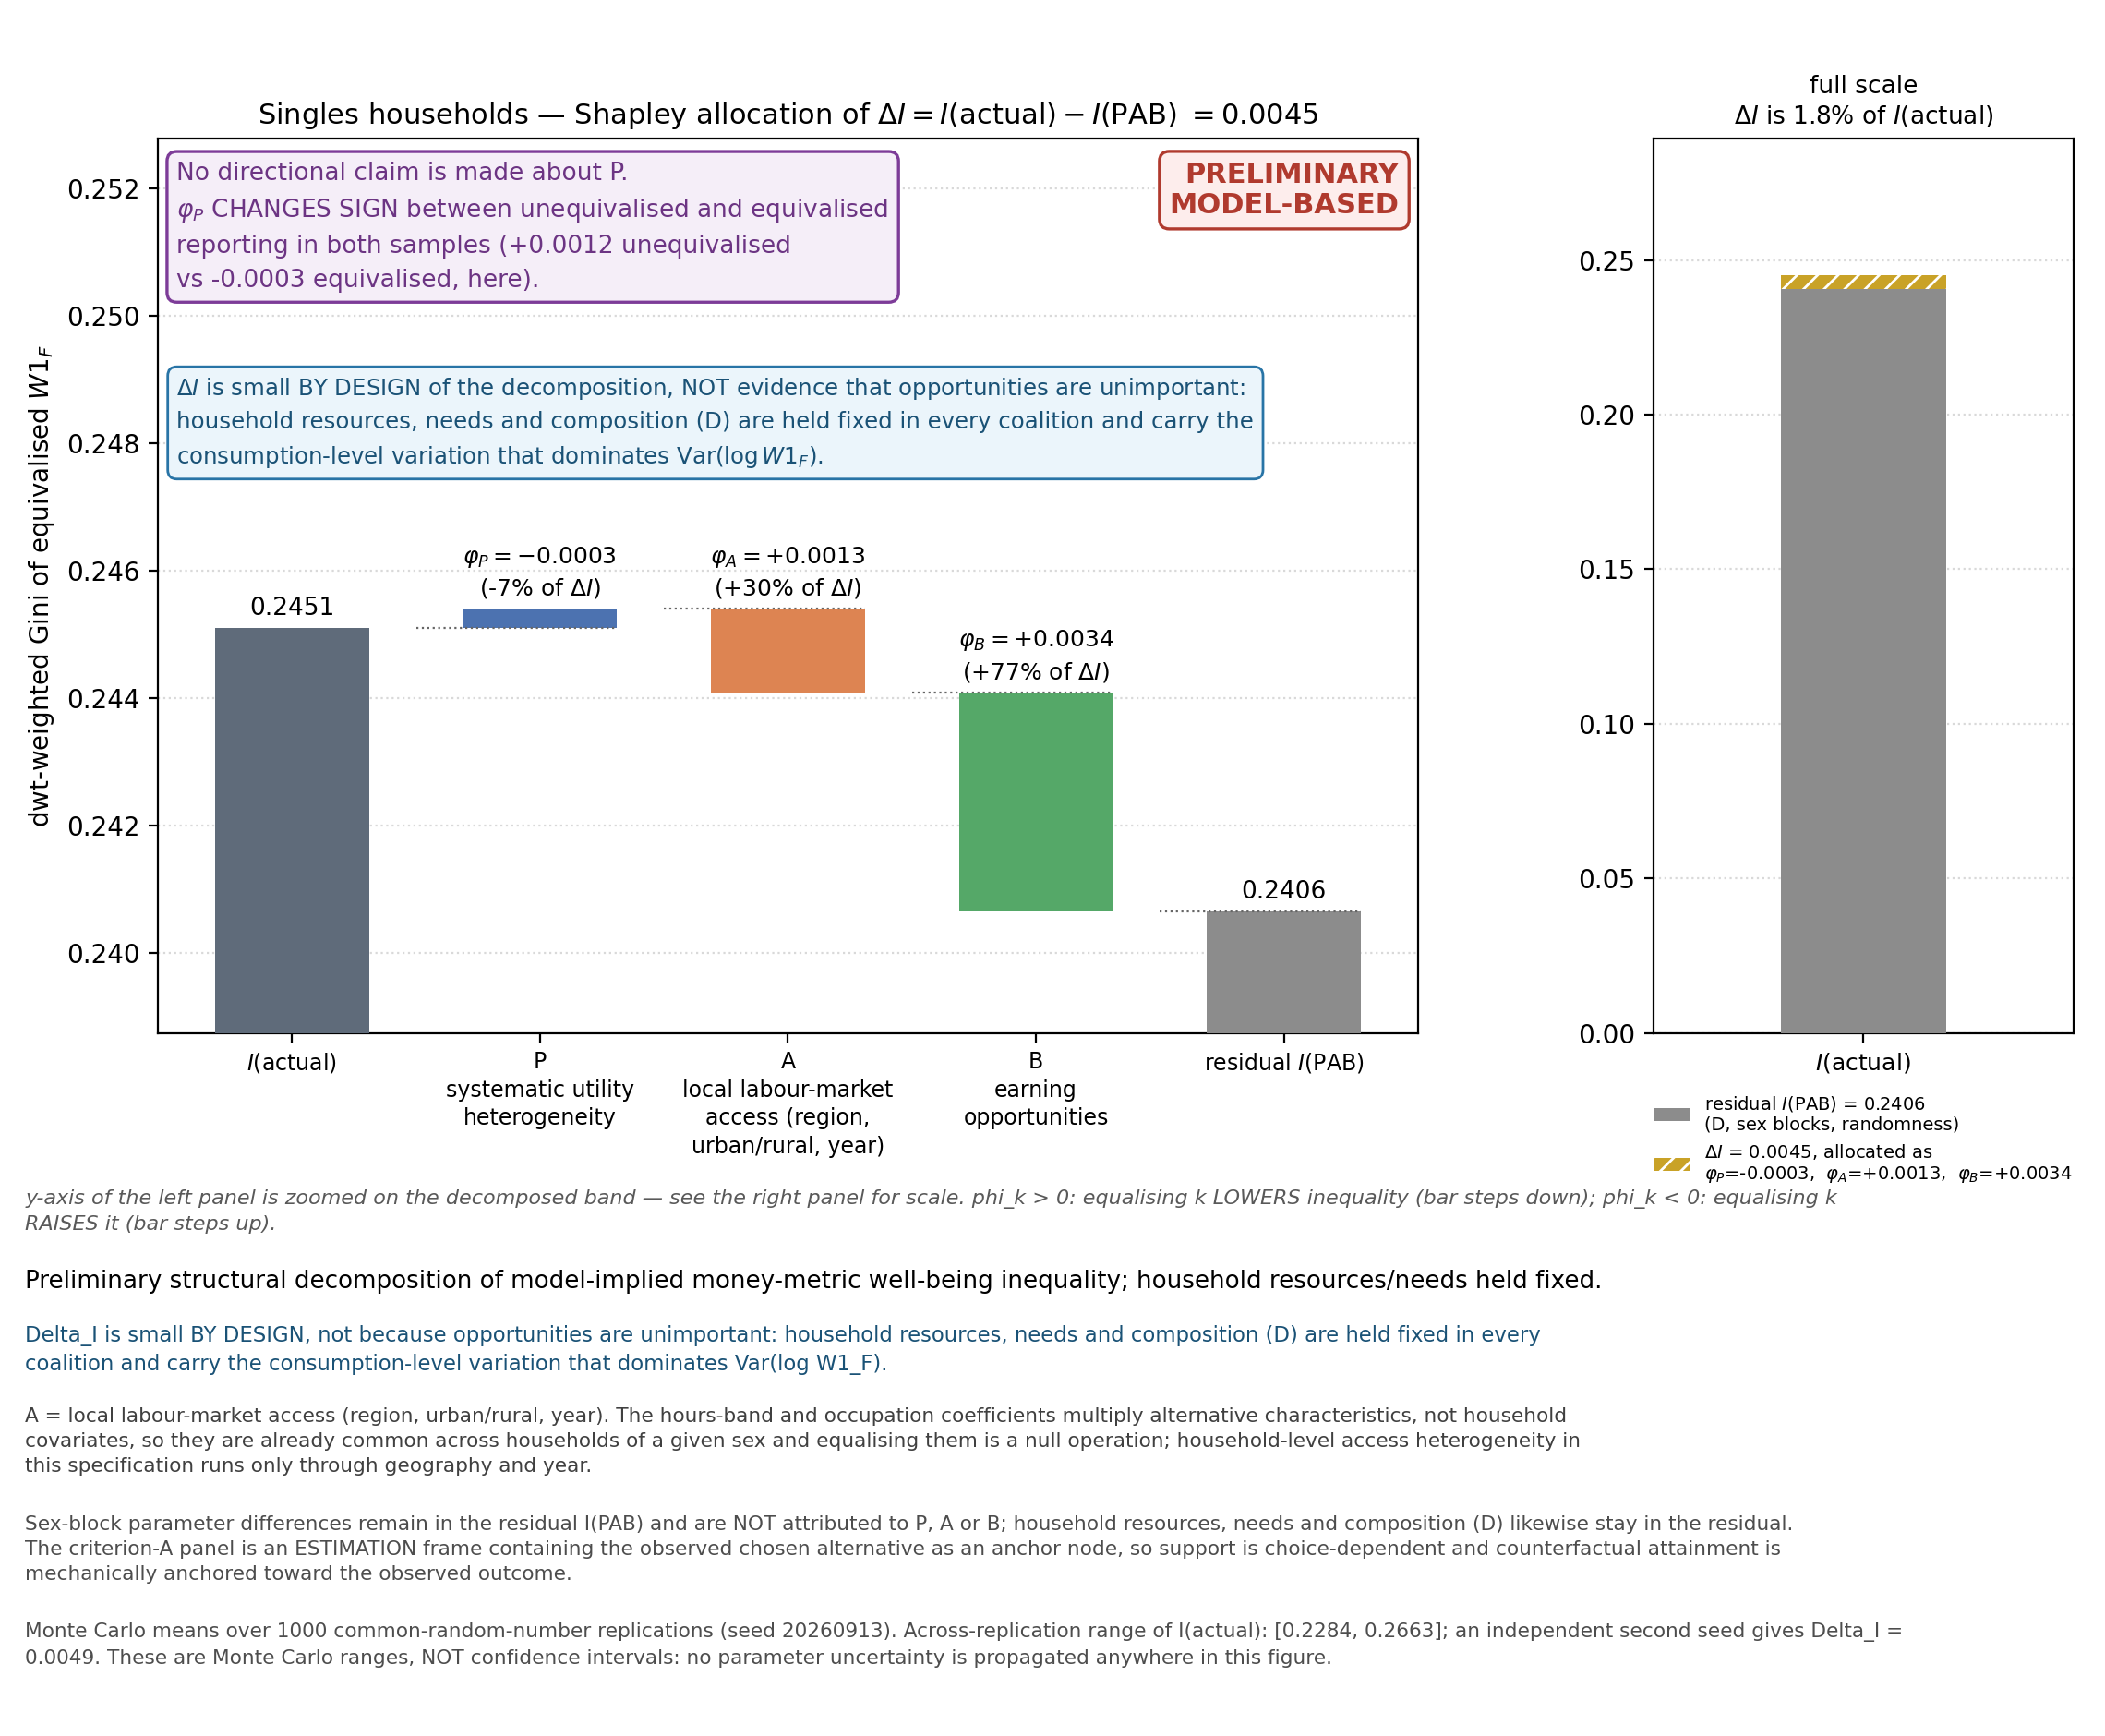
\includegraphics[width=0.95\linewidth,height=\textheight,keepaspectratio,alt={Single-adult estimation sample: coalition Gini levels and the exact Shapley allocation of \textbackslash Delta I across P, A and B, with the sign instability of P annotated. Modified-OECD-equivalised W\^{}1\_F; Monte Carlo ranges over 1,000 replications, not confidence intervals. Preliminary, model-based.}]{figures/v5/fig_preseminar_pab_decomposition_singles_v1.png}
\caption{Single-adult estimation sample: coalition Gini levels and the exact Shapley allocation of \(\Delta I\) across P, A and B, with the sign instability of P annotated. Modified-OECD-equivalised \(W^1_F\); Monte Carlo ranges over 1,000 replications, not confidence intervals. Preliminary, model-based.}
\end{figure}

\begin{figure}[H]
\centering
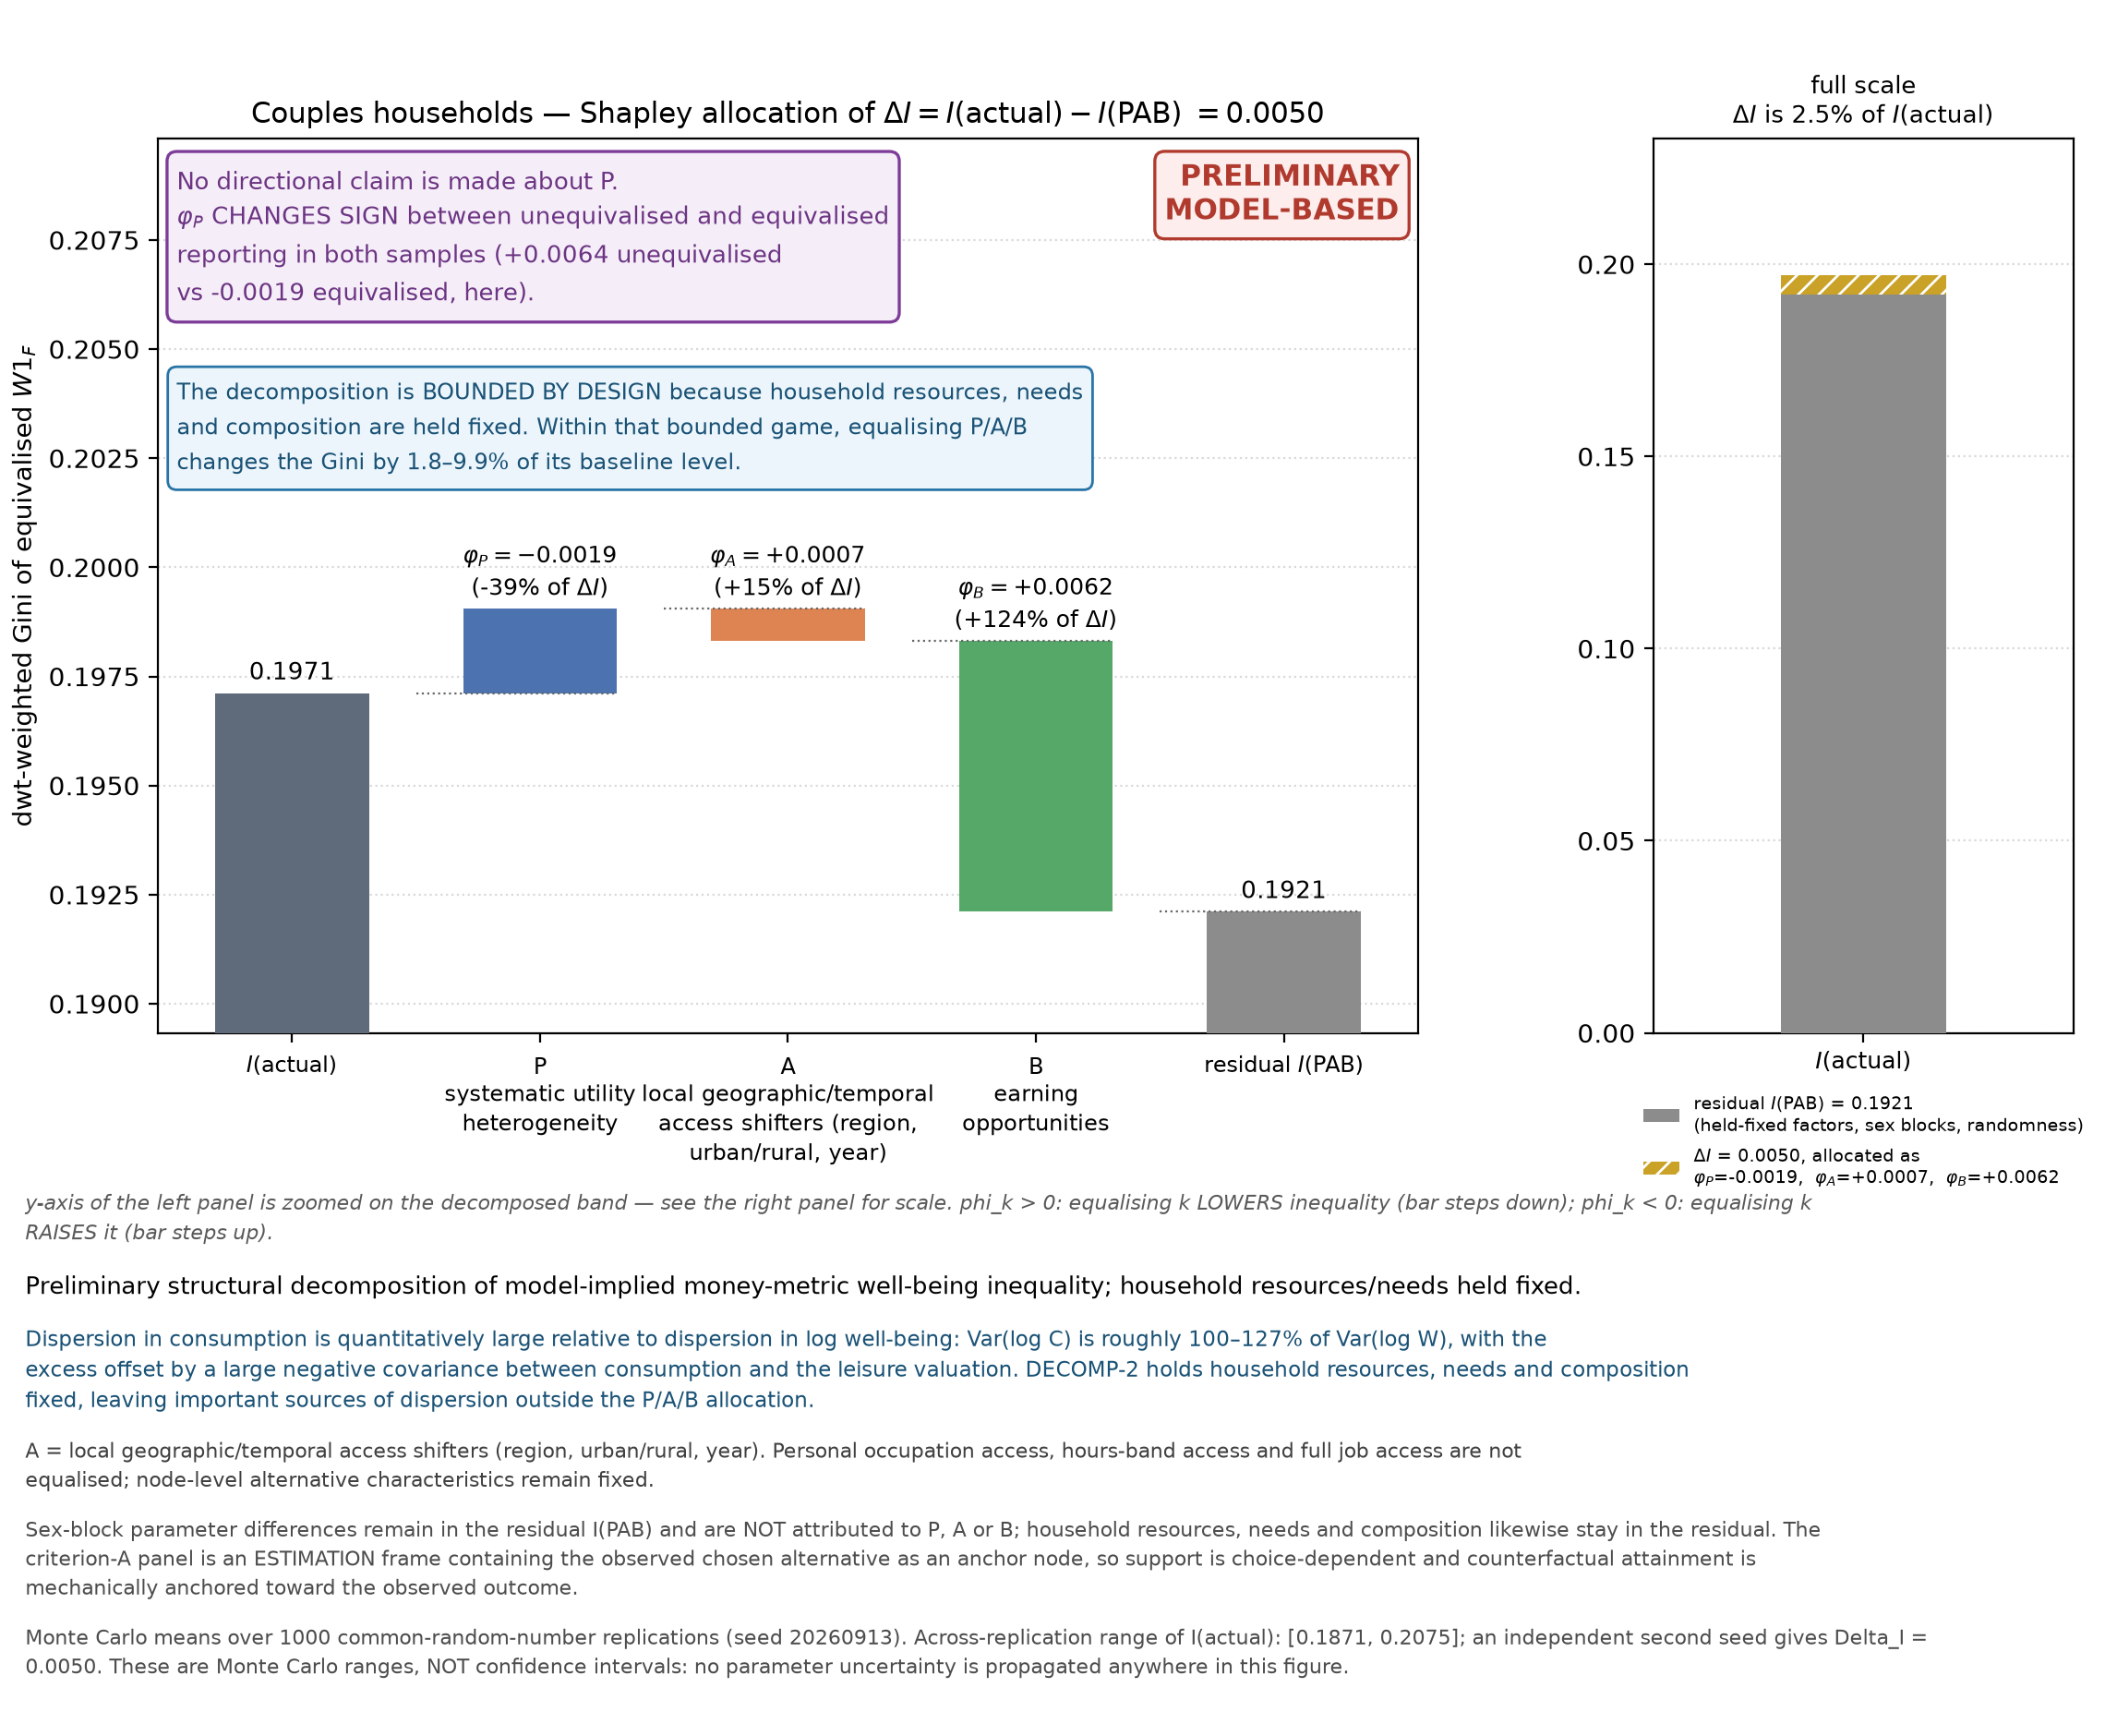
\includegraphics[width=0.95\linewidth,height=\textheight,keepaspectratio,alt={Couple estimation sample: coalition Gini levels and the exact Shapley allocation of \textbackslash Delta I across P, A and B, with the sign instability of P annotated. Modified-OECD-equivalised W\^{}1\_F; Monte Carlo ranges over 1,000 replications, not confidence intervals. Preliminary, model-based.}]{figures/v5/fig_preseminar_pab_decomposition_couples_v1.png}
\caption{Couple estimation sample: coalition Gini levels and the exact Shapley allocation of \(\Delta I\) across P, A and B, with the sign instability of P annotated. Modified-OECD-equivalised \(W^1_F\); Monte Carlo ranges over 1,000 replications, not confidence intervals. Preliminary, model-based.}
\end{figure}

In a preliminary three-factor structural exercise that holds household resources, needs and composition fixed, equalising systematic utility heterogeneity, coarse geographic/temporal access heterogeneity and earning opportunities changes money-metric well-being inequality by 1.8--9.9\% of the baseline Gini, depending on household type and reporting scale. Within the Shapley allocation of that movable component, earning-opportunity heterogeneity has a larger contribution than the coarse geographic/temporal access channel in both samples and both reporting conventions. The preference contribution is not sign-robust to equivalisation.

These are preliminary model-based accounting results, not causal estimates and not the final decomposition of total well-being inequality.

The allocated shares are not one-factor effects. An allocated share is an average of marginal contributions over the orders in which coalitions can form; the coalition table above reports the one-factor effect directly, as the change from the actual coalition for the single-letter row. The two can differ, and with three players and an exact Shapley value the difference is fully accounted for by the interaction terms, which the closed form makes explicit.

\textbf{Robustness.} Every coalition Gini level and every Shapley contribution reproduces closely under an independent second simulation seed, including the sign instability of the preference contribution, which appears in both runs. Excluding the estimation panel's anchor node -- the household's own observed choice, inserted deterministically in every coalition, which mechanically anchors counterfactual attainment toward the observed outcome to a small, roughly common degree (2.9 per cent of single adults and 3.9 per cent of couples attain it under any coalition) -- moves \(\Delta I\) by at most 9.3 per cent (couples, equivalised), with no sign flip in any specification.

The allocation is exhaustive to numerical precision: the residual after summing \(P\), \(A\), \(B\) and \(\Delta I\) back to \(I_\varnothing\) is zero to machine precision in every sample and scale, verified rather than imposed. That is a computational validation of the accounting for the declared game. It does not validate the identification of the model, the normative content of the operators, or a resolution of the counterfactual-attainment question this exercise is deliberately bounded around.

\subsection{Equivalization and the preliminary decomposition}\label{equivalization-and-the-preliminary-decomposition}

Equivalization is a normative choice, and the preliminary decomposition in Appendix D moves with it. On the equivalized basis the movable share \(\Delta I\) is larger relative to baseline inequality for both household types than on the raw household basis, and the earning-opportunities/coarse-geographic-and-temporal-access ordering is unchanged in every case: earning opportunities have the larger contribution at both scales, for both household types. The preference contribution's sign already differs between the two scales at the raw comparison reported in Appendix D; equivalization is one of the two axes that sign instability spans, not an independent further concern. Both bases are reported throughout; neither is the correct one, and the choice between them is not settled by the data. We do not report a male-primary or other alternative reference-block variant of this preliminary exercise; that sensitivity, reported for the welfare baseline itself in Section 4, has not been re-run through the bounded decomposition.

\textbf{The \(A\) channel is local geographic/temporal access only.} The operator \(A_i\) of Section 4 carries region, urban/rural status and survey year; it does not carry any individual capability, education-specific or occupation-specific access channel, hours-band access or full job access. What the preliminary decomposition attributes to \(A\) is therefore the coarse geographic and temporal component of access, not access in the fuller sense of what an individual with particular skills or credentials can reach; a more personal access channel, if identified, would move some inequality currently attributed elsewhere into \(A\), in a direction we do not sign.

\textbf{\(\Delta I\) is bounded by design.} The decomposition is bounded by design because household resources, needs and composition are held fixed. Within that bounded game, equalising P/A/B changes the Gini by 1.8--9.9\% of its baseline level, depending on sample and reporting scale. The restriction is by construction; the realised numerical magnitude is a model result under that restriction.

\textbf{The preference contribution's sign depends on the reporting scale.} \(\phi_P\), the exact Shapley contribution of preferences, changes sign between the unequivalised and equivalised reporting conventions in both samples. We therefore make no directional claim about the preference contribution, only about the ordering of the coarse geographic/temporal access channel against earning opportunities, which is scale-robust.

The appendix decomposition is bounded and preliminary in three specific ways, stated together here. It holds household resources, needs and composition fixed rather than decomposing them, leaving important sources of dispersion outside the P/A/B allocation; the reported 1.8--9.9\% change is defined within that bounded game. It reuses the model's already-priced estimation panel to simulate counterfactual attainment, which anchors that attainment toward the observed outcome to a small, checked degree, rather than resolving the counterfactual-attainment estimand the paper's final decomposition architecture requires. And its uncertainty is reported as a Monte Carlo simulation range and an independent second-seed check, not as a parameter-uncertainty interval propagated from the estimation covariance. None of the three is a defect in what is reported; together they are why it is reported as preliminary rather than as the paper's decomposition result.

\subsection{Interpretation of the restricted results}\label{interpretation-of-the-restricted-results}

The normative half then yields, for each household, an equivalent flat consumption level. Attributing its inequality to preferences and to circumstances in full requires a counterfactual-attainment estimand for the bundle a household would attain under a counterfactual environment, and that estimand is still under design. Ahead of it we report a bounded, preliminary exercise: we define three structural equalization operators, one for systematic utility heterogeneity, one for coarse geographic/temporal access heterogeneity and one for earning opportunities, holding household resources, needs and composition fixed throughout; we recompute every household's welfare level, and the inequality of the resulting distribution, under each of the eight coalitions of those three operators, reusing the model's own already-priced estimation panel with no re-estimation and no new pricing; and we allocate the interactions among them with an exact three-player Shapley value. The allocation is exhaustive by construction and the closure is verified numerically rather than imposed.

\textbf{Restricted results.} In a preliminary three-factor structural exercise that holds household resources, needs and composition fixed, equalising systematic utility heterogeneity, coarse geographic/temporal access heterogeneity and earning opportunities changes money-metric well-being inequality by 1.8--9.9\% of the baseline Gini, depending on household type and reporting scale. Within the Shapley allocation of that movable component, earning-opportunity heterogeneity has a larger contribution than the coarse geographic/temporal access channel in both samples and both reporting conventions. The preference contribution is not sign-robust to equivalisation. These are preliminary model-based accounting results, not causal estimates and not the final decomposition of total well-being inequality.

Two qualifications belong with these appendix results. First, the preference contribution's sign is not robust between the unequivalised and equivalised reporting conventions, in either sample: we therefore make no directional claim about it, only about the ordering of access against earnings. Second, an allocated share is an average of marginal contributions over coalition orders. It is not the reduction that equalizing that factor alone would achieve; Appendix D reports both and explains why they can differ, and reports the exact scale at which excluding the model's anchored-attainment arm moves \(\Delta I\), as a robustness check on the design rather than on the estimates. This is a bounded, preliminary reading, reported ahead of the paper's final decomposition architecture, and it should be read as such throughout.

\section{Scientific history of this result}\label{scientific-history-of-this-result}

This section records how the reported specifications and results came to be what they are. It is here so that the argument above does not have to carry it, and so that a reader comparing this version with an earlier one can see what changed and why. Nothing in it is a competing model.

\textbf{The consumption specification.} Earlier drafts reported a specification in which the consumption coefficient was fixed as a numeraire, and one in which the single-adult consumption curvature was estimated rather than fixed. Neither is the reported model. The current specification fixes the shock scale, fixes the consumption curvature at exactly zero, and estimates the consumption weight instead. That change improves the criterion by 23.753 log-points for single adults and 15.659 for couples, and it changes how a given non-consumption advantage converts into the money metric: under the closed form of Section 4, that advantage now enters divided by the estimated \(\beta_c\) rather than by the fixed numeraire it previously used. Every welfare quantity computed under the earlier convention is superseded, and the corresponding figures were regenerated rather than relabelled.

\textbf{The sample.} The predecessor frames were screened further when the hours support and occupation mapping were applied to observed rows, with a further exclusion where an observed job prices to non-positive disposable consumption. The current descriptive tables are computed on the resulting 1,540 and 2,223 households, not on the predecessor frames, and the funnel in Section 2 ends where the estimation begins.

\textbf{The disposable-income convention.} Single-adult disposable income was previously aggregated over the decider only; it is now aggregated over all resident household members, which is the convention the couples application always used. The two applications are now on the same accounting convention.

\textbf{The decomposition result.} Appendix D reports only the bounded, explicitly preliminary three-factor exercise: systematic utility heterogeneity, coarse geographic/temporal access shifters and earning opportunities, with resources, needs and composition held fixed. It is based on a full recomputation of the bounded exercise and reported with Monte Carlo simulation ranges and a second-seed check rather than parameter-uncertainty intervals. Earlier architectures and their numerical results are absent from every current reader-facing surface and remain only in the audit record.

\textbf{The welfare reference.} Section 4 reports only the own-set equal-consumption construction with the universally available non-employment state as its reference. Under the current specification the home reference carries no opportunity-density, proposal, shock or intensity argument. Superseded candidates and their numerical results are absent from every current reader-facing surface and remain only in the audit record.

\textbf{The consumption normalizer.} Three values of \(\lambda_c\) were in circulation because different panels recomputed it over their own rows. Under exact log consumption the constant is alternative-invariant and cancels from every choice probability; it does not enter the \(W^1_F\) welfare measure at all, so no welfare result is affected by which value is used. The paper now reports one constant per population, for the choice-probability role it actually plays.

\bibliographystyle{plainnat}
\bibliography{JMP_working_paper_for_seminar_v6}
% BEGIN READER-VOICE PROVENANCE
% Source-only provenance; excluded from rendered reader text.
% Specifications: S11; artifact s11_welfare_specs_of_record_v1.json; SHA-256 5FDC88502493CE540B088880EECF049BC268392FF3E8790FFE78A16AA6DDC884.
% Welfare definition: Mapping F; artifact JMP_W1_fork_ruling_v1.md; SHA-256 7F5D26857D8A96174A9924848F65A02611944273D7775FDC52DC82364A818C05.
% Welfare authorization: BASELINE-F-1 and E1; artifact JMP_W1_BASELINE_F1_authorization_and_Cobs_ruling_v1.md; SHA-256 54DFD886E41D0A89C1056CBEA5FA51E0A1294D3CA0813F938802BDC3DBD9EE0E.
% Welfare aggregates: artifact baseline_f1_verification_v1.md; MNL commit 6048c9f7; independent verification b5550af5; SHA-256 DA7BADF639F3D502D47B301558453D76501C9C44033ECE3F17BDE350BFD5E55F.
% Equivalised reporting: E3-EQ; artifact JMP_BASELINE_F1_equivalised_reporting_v1.md; commit 4c4e07e; SHA-256 DACD34B593D0E676AC802779960DBB4F4BDC32A462C26F8852D56C9D4C95A669.
% Predictive diagnostics: POSFIT v3; repository MNL_posfit; branch diagnostics/posfit-v3; commit 96693269; artifact run_provenance.json; SHA-256 BDC3722C325FF8A27BE719AA52A741DF7BEEF9515B4A63554C65E8769EB7F40B.
% Bounded decomposition: DECOMP-2; repository MNL_decomp; branch welfare/preseminar-pab; commit b52761b4; artifact preseminar_pab_record_v1.json; SHA-256 BCBE4B6FC742DAA39535D5C3EB03BDA0641055A9F5E851B4F53F62FA3E612011.
% Leisure scaling: WS4; commit 5a8e6bba; artifacts ws4_sectionC_lambda_v1.png and ws4_sectionC_T_v1.png.
% Diagnostic boundary: DECOMP-DIAG-1; artifact docs/Decomposition_diag_1.txt; SHA-256 EAD1B7C8243FE1498F00DCF287331BEEC94165332AA3BB64041A0F645D339A74.
% REPORT-V6: presentation-only successor; frozen v5 tables, figures and scalar values.
% END READER-VOICE PROVENANCE
\end{document}
